\documentclass{beamer}
\usefonttheme[onlymath]{serif}
\usepackage[T1]{fontenc}
\usepackage[utf8]{inputenc}
\usepackage[english]{babel}
\usepackage{amsmath}
\usepackage{amssymb}
\usepackage{amsthm}
\usepackage{gensymb}
\usepackage{parskip}
\usepackage{mathtools}
\usepackage{listings}
\usepackage{hyperref}
\usepackage{graphicx}
\usepackage{color}
\usepackage{enumerate}
\usepackage{tikz}
\usetikzlibrary{calc}
\usetikzlibrary{positioning}
\usetikzlibrary{angles}
\usetikzlibrary{shapes}
\usetikzlibrary{arrows}
\usepackage{verbatim}
\usepackage{multicol}
\usepackage{array}
\usepackage{minted}
\parskip 0pt

\usepackage{colortbl}
\usepackage{pgf}
\usepackage{pgfkeys}
\usetikzlibrary{fpu}
\usepackage{tkz-euclide}

\DeclareMathOperator{\lcm}{lcm}
\newcommand\floor[1]{\left\lfloor#1\right\rfloor}
\newcommand\ceil[1]{\left\lceil#1\right\rceil}
\newcommand\abs[1]{\left|#1\right|}
\newcommand\p[1]{\left(#1\right)}
\newcommand\sqp[1]{\left[#1\right]}
\newcommand\cp[1]{\left\{#1\right\}}
\newcommand\norm[1]{\left\lVert#1\right\rVert}
\renewcommand\Im{\operatorname{Im}}
\renewcommand\Re{\operatorname{Re}}

\usetheme{metropolis}
\definecolor{dark yellow}{rgb} {0.6,0.6,0.0}
\definecolor{dark green}{rgb} {0.0,0.6,0.0}

\graphicspath{{myndir/}}

\tikzstyle{vertex}=[circle,fill=black!50,minimum size=15pt,inner sep=0pt, font=\small]
\tikzstyle{selected vertex} = [vertex, fill=red!24]
\tikzstyle{edge} = [draw,thick,-]
\tikzstyle{dedge} = [draw,thick,->]
\tikzstyle{weight} = [font=\scriptsize,pos=0.5]
\tikzstyle{selected edge} = [draw,line width=2pt,-,red!50]
\tikzstyle{selected2 vertex} = [vertex, fill=hilight!50, text=black]
\tikzstyle{ignored edge} = [draw,line width=5pt,-,black!20]
\tikzstyle{vertex1} = [vertex, fill=red]
\tikzstyle{vertex2} = [vertex, fill=blue]
\tikzstyle{vertex3} = [vertex, fill=green, text=black]
\tikzstyle{vertex4} = [vertex, fill=yellow, text=black]
\tikzstyle{vertex5} = [vertex, fill=pink, text=black]
\tikzstyle{vertex6} = [vertex, fill=purple]

\tikzset{
	treenode/.style = {align=center, inner sep=0pt, text centered,
		font=\sffamily},
	vertex/.style = {treenode, circle, black, font=\sffamily\bfseries\tiny, draw=black, text width=1.8em},% arbre rouge noir, noeud noir
	rvertex/.style = {treenode, circle, black, font=\sffamily\bfseries\tiny, draw=red, text width=1.8em},% arbre rouge noir, noeud noir
}

\definecolor{offwhite}{RGB}{249,242,215}
\definecolor{foreground}{HTML}{23373b}
\definecolor{background}{RGB}{24,24,24}
\definecolor{title}{RGB}{107,174,214}
\definecolor{gray}{RGB}{155,155,155}
\definecolor{subtitle}{RGB}{102,255,204}
\definecolor{lolight}{RGB}{155,155,155}
\definecolor{green}{RGB}{125,250,125}

\definecolor{hilight}{RGB}{235,129,27}
\definecolor{vhilight}{HTML}{14B03D}

\def\hepta{\draw[foreground](A) -- (B) -- (C) -- (D) -- (E) -- (F) -- (G) -- cycle;}

\newcommand{\slice}[1]{%
	\hepta
	\draw[foreground] \foreach \x/\y in {#1} {(\x)--(\y)};
}

\title{Graphs Part 3}
\author{Atli Fannar Franklín}
\institute{\href{http://ru.is/td}{School of Computer Science} \\[2pt] \href{http://ru.is}{Reykjavík University}}
\titlegraphic{\hfill
\includegraphics[height=0.6cm]{kattis}}

\begin{document}
	\maketitle
	
	\begin{frame}[plain]{Today we're going to cover}
		\begin{itemize}
			\item Maximum flow
			\begin{itemize}
				\item Ford-Fulkerson
				\item Edmond-Karp
				\item Dinic's
				\item MCMF
			\end{itemize}
		\end{itemize}
	\end{frame}
	
	\begin{frame}[plain]{Flow problems}
		\begin{itemize}
			\item What is maximum flow?
			\item We imagine each edge in a (directed) graph is a pipe, and the weight says how many units of liquid can pass through it per second.
			\item Then vertices are joints, and the amount of liquid going in and out must be the same.
			\item Except for one vertex where we let water flow in from the outside, the source, and one where we let it flow out, the sink.
			\item Then the maximum flow problem is the problem of determining the maximum amount of liquid that can flow per second from the source to the sink.
		\end{itemize}
	\end{frame}
	
	\begin{frame}[plain]{Formal definition}
		\begin{itemize}
			\item For a graph $G = (V, E)$ we say that $f : E \rightarrow \mathbb{R}$ is a flow from $s \in V$ to $t \in V$ if $0 \leq f(e) \leq c_e$ where $c_e$ is the capacity for $e$ and for all $v \in V \setminus{s, t}$ we have
			\[\sum_{e \in \text{out}(v)} f(e) = \sum_{e \in \text{in}(v)} f(e)\]
			\item The value of a flow $f$ is the amount of liquid flowing out at the source (or in at the sink, equivalently), more formally given as
			\[\sum_{e \in \text{out}(s)} f(e) = \sum_{e \in \text{in}(t)} f(e)\]
			\item The maximum flow problem is then to find the flow with the maximum value for a given graph.
		\end{itemize}
	\end{frame}
	
	\begin{frame}[plain]{First solution ideas}
		\begin{itemize}
			\item How do we solve this?
			\item Brute force trying every combination will be massively slow.
			\item So we just try something greedy.
			\item<2-> How about we just find some path from $s$ to $t$ where we can fit more flow, and fit more flow there?
			\item<2-> Rinse and repeat, until we get stuck.
		\end{itemize}
	\end{frame}
	
	\begin{frame}[plain]{Example}
		\begin{center}
			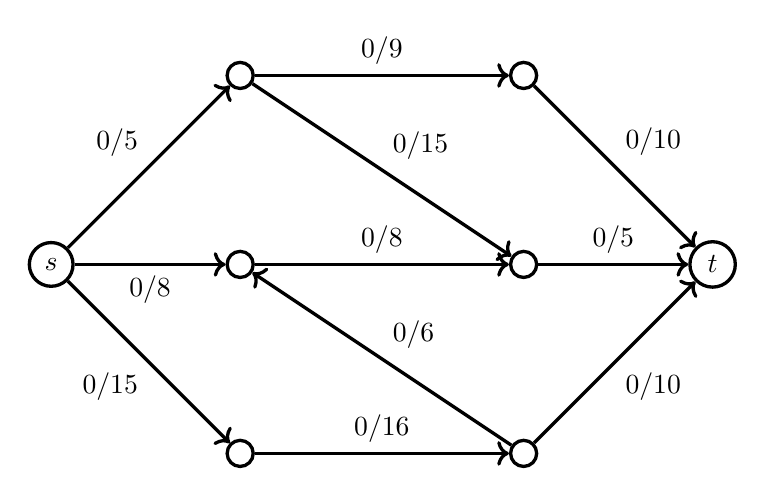
\begin{tikzpicture}[scale=1.2]
				\node[circle, draw, very thick] (0) at (0,0) {$s$};
				\node[circle, draw, very thick] (1) at (2,-2) {};
				\node[circle, draw, very thick] (2) at (2,0) {};
				\node[circle, draw, very thick] (3) at (2,2) {};
				\node[circle, draw, very thick] (4) at (5,-2) {};
				\node[circle, draw, very thick] (5) at (5,0) {};
				\node[circle, draw, very thick] (6) at (5,2) {};
				\node[circle, draw, very thick] (7) at (7,0) {$t$};
				
				\draw[very thick, ->]  (0) -- (1) node[midway,below left] () {$0/15$};
				\draw[very thick, ->]  (0) -- (2) node[midway,below] () {$0/8$};
				\draw[very thick, ->]  (0) -- (3) node[midway,above left] () {$0/5$};
				\draw[very thick, ->]  (1) -- (4) node[midway,above] () {$0/16$};
				\draw[very thick, ->]  (2) -- (5) node[midway,above] () {$0/8$};
				\draw[very thick, ->]  (3) -- (6) node[midway,above] () {$0/9$};
				\draw[very thick, ->]  (3) -- (5) node[midway,above right] () {$0/15$};
				\draw[very thick, ->]  (4) -- (2) node[midway,above right] () {$0/6$};
				\draw[very thick, ->]  (4) -- (7) node[midway,below right] () {$0/10$};
				\draw[very thick, ->]  (5) -- (7) node[midway,above] () {$0/5$};
				\draw[very thick, ->]  (6) -- (7) node[midway,above right] () {$0/10$};
			\end{tikzpicture}
		\end{center}
	\end{frame}
	
	\begin{frame}[plain]{Example}
		\begin{center}
			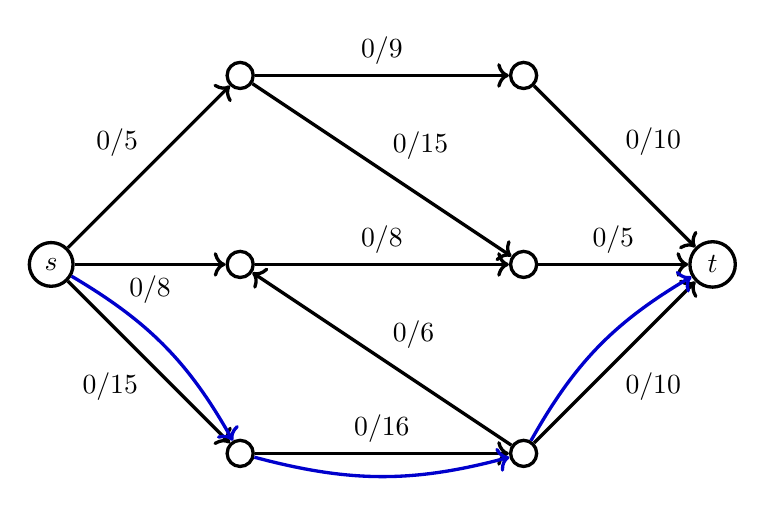
\begin{tikzpicture}[scale=1.2]
				\node[circle, draw, very thick] (0) at (0,0) {$s$};
				\node[circle, draw, very thick] (1) at (2,-2) {};
				\node[circle, draw, very thick] (2) at (2,0) {};
				\node[circle, draw, very thick] (3) at (2,2) {};
				\node[circle, draw, very thick] (4) at (5,-2) {};
				\node[circle, draw, very thick] (5) at (5,0) {};
				\node[circle, draw, very thick] (6) at (5,2) {};
				\node[circle, draw, very thick] (7) at (7,0) {$t$};
				
				\draw[very thick, ->]  (0) -- (1) node[midway,below left] () {$0/15$};
				\draw[very thick, ->]  (0) -- (2) node[midway,below] () {$0/8$};
				\draw[very thick, ->]  (0) -- (3) node[midway,above left] () {$0/5$};
				\draw[very thick, ->]  (1) -- (4) node[midway,above] () {$0/16$};
				\draw[very thick, ->]  (2) -- (5) node[midway,above] () {$0/8$};
				\draw[very thick, ->]  (3) -- (6) node[midway,above] () {$0/9$};
				\draw[very thick, ->]  (3) -- (5) node[midway,above right] () {$0/15$};
				\draw[very thick, ->]  (4) -- (2) node[midway,above right] () {$0/6$};
				\draw[very thick, ->]  (4) -- (7) node[midway,below right] () {$0/10$};
				\draw[very thick, ->]  (5) -- (7) node[midway,above] () {$0/5$};
				\draw[very thick, ->]  (6) -- (7) node[midway,above right] () {$0/10$};
				
				\draw[very thick, blue!80!black, ->] (0) to [bend left=15] (1);
				\draw[very thick, blue!80!black, ->] (1) to [bend right=15] (4);
				\draw[very thick, blue!80!black, ->] (4) to [bend left=15] (7);
			\end{tikzpicture}
		\end{center}
	\end{frame}
	
	\begin{frame}[plain]{Example}
		\begin{center}
			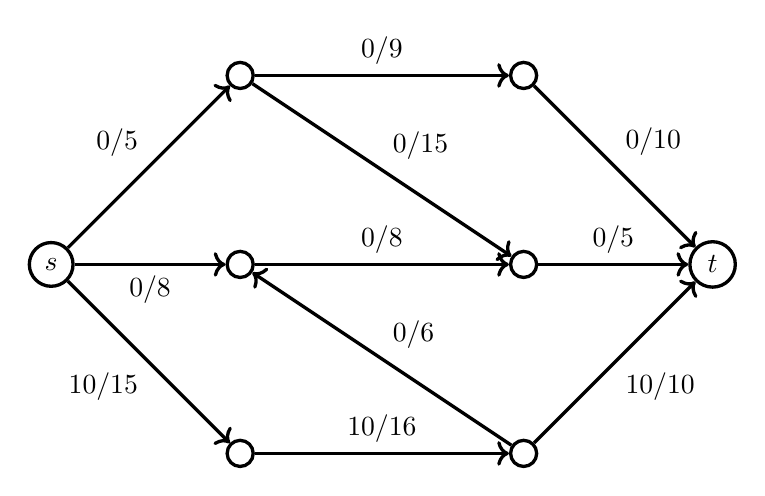
\begin{tikzpicture}[scale=1.2]
				\node[circle, draw, very thick] (0) at (0,0) {$s$};
				\node[circle, draw, very thick] (1) at (2,-2) {};
				\node[circle, draw, very thick] (2) at (2,0) {};
				\node[circle, draw, very thick] (3) at (2,2) {};
				\node[circle, draw, very thick] (4) at (5,-2) {};
				\node[circle, draw, very thick] (5) at (5,0) {};
				\node[circle, draw, very thick] (6) at (5,2) {};
				\node[circle, draw, very thick] (7) at (7,0) {$t$};
				
				\draw[very thick, ->]  (0) -- (1) node[midway,below left] () {$10/15$};
				\draw[very thick, ->]  (0) -- (2) node[midway,below] () {$0/8$};
				\draw[very thick, ->]  (0) -- (3) node[midway,above left] () {$0/5$};
				\draw[very thick, ->]  (1) -- (4) node[midway,above] () {$10/16$};
				\draw[very thick, ->]  (2) -- (5) node[midway,above] () {$0/8$};
				\draw[very thick, ->]  (3) -- (6) node[midway,above] () {$0/9$};
				\draw[very thick, ->]  (3) -- (5) node[midway,above right] () {$0/15$};
				\draw[very thick, ->]  (4) -- (2) node[midway,above right] () {$0/6$};
				\draw[very thick, ->]  (4) -- (7) node[midway,below right] () {$10/10$};
				\draw[very thick, ->]  (5) -- (7) node[midway,above] () {$0/5$};
				\draw[very thick, ->]  (6) -- (7) node[midway,above right] () {$0/10$};
			\end{tikzpicture}
		\end{center}
	\end{frame}
	
	\begin{frame}[plain]{Example}
		\begin{center}
			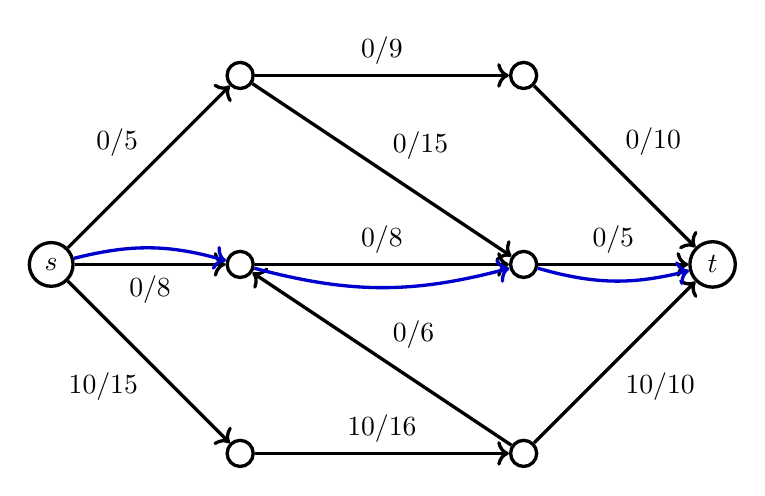
\begin{tikzpicture}[scale=1.2]
				\node[circle, draw, very thick] (0) at (0,0) {$s$};
				\node[circle, draw, very thick] (1) at (2,-2) {};
				\node[circle, draw, very thick] (2) at (2,0) {};
				\node[circle, draw, very thick] (3) at (2,2) {};
				\node[circle, draw, very thick] (4) at (5,-2) {};
				\node[circle, draw, very thick] (5) at (5,0) {};
				\node[circle, draw, very thick] (6) at (5,2) {};
				\node[circle, draw, very thick] (7) at (7,0) {$t$};
				
				\draw[very thick, ->]  (0) -- (1) node[midway,below left] () {$10/15$};
				\draw[very thick, ->]  (0) -- (2) node[midway,below] () {$0/8$};
				\draw[very thick, ->]  (0) -- (3) node[midway,above left] () {$0/5$};
				\draw[very thick, ->]  (1) -- (4) node[midway,above] () {$10/16$};
				\draw[very thick, ->]  (2) -- (5) node[midway,above] () {$0/8$};
				\draw[very thick, ->]  (3) -- (6) node[midway,above] () {$0/9$};
				\draw[very thick, ->]  (3) -- (5) node[midway,above right] () {$0/15$};
				\draw[very thick, ->]  (4) -- (2) node[midway,above right] () {$0/6$};
				\draw[very thick, ->]  (4) -- (7) node[midway,below right] () {$10/10$};
				\draw[very thick, ->]  (5) -- (7) node[midway,above] () {$0/5$};
				\draw[very thick, ->]  (6) -- (7) node[midway,above right] () {$0/10$};
				
				\draw[very thick, blue!80!black, ->] (0) to [bend left=15] (2);
				\draw[very thick, blue!80!black, ->] (2) to [bend right=15] (5);
				\draw[very thick, blue!80!black, ->] (5) to [bend right=15] (7);
			\end{tikzpicture}
		\end{center}
	\end{frame}
	
	\begin{frame}[plain]{Example}
		\begin{center}
			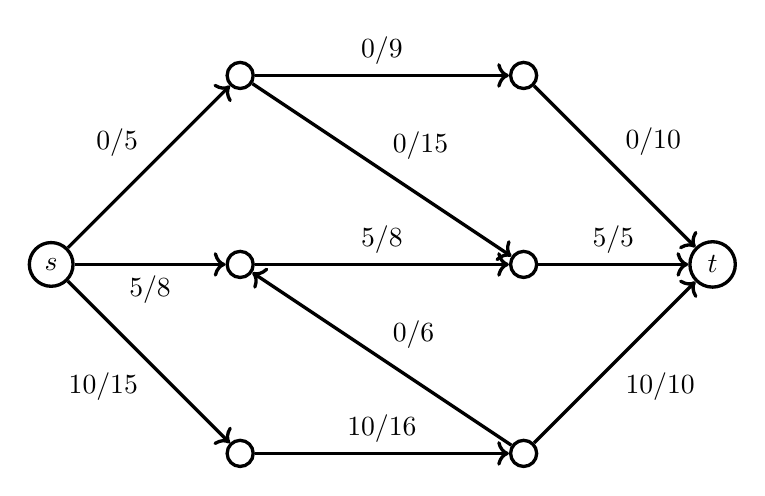
\begin{tikzpicture}[scale=1.2]
				\node[circle, draw, very thick] (0) at (0,0) {$s$};
				\node[circle, draw, very thick] (1) at (2,-2) {};
				\node[circle, draw, very thick] (2) at (2,0) {};
				\node[circle, draw, very thick] (3) at (2,2) {};
				\node[circle, draw, very thick] (4) at (5,-2) {};
				\node[circle, draw, very thick] (5) at (5,0) {};
				\node[circle, draw, very thick] (6) at (5,2) {};
				\node[circle, draw, very thick] (7) at (7,0) {$t$};
				
				\draw[very thick, ->]  (0) -- (1) node[midway,below left] () {$10/15$};
				\draw[very thick, ->]  (0) -- (2) node[midway,below] () {$5/8$};
				\draw[very thick, ->]  (0) -- (3) node[midway,above left] () {$0/5$};
				\draw[very thick, ->]  (1) -- (4) node[midway,above] () {$10/16$};
				\draw[very thick, ->]  (2) -- (5) node[midway,above] () {$5/8$};
				\draw[very thick, ->]  (3) -- (6) node[midway,above] () {$0/9$};
				\draw[very thick, ->]  (3) -- (5) node[midway,above right] () {$0/15$};
				\draw[very thick, ->]  (4) -- (2) node[midway,above right] () {$0/6$};
				\draw[very thick, ->]  (4) -- (7) node[midway,below right] () {$10/10$};
				\draw[very thick, ->]  (5) -- (7) node[midway,above] () {$5/5$};
				\draw[very thick, ->]  (6) -- (7) node[midway,above right] () {$0/10$};
			\end{tikzpicture}
		\end{center}
	\end{frame}
	
	\begin{frame}[plain]{Example}
		\begin{center}
			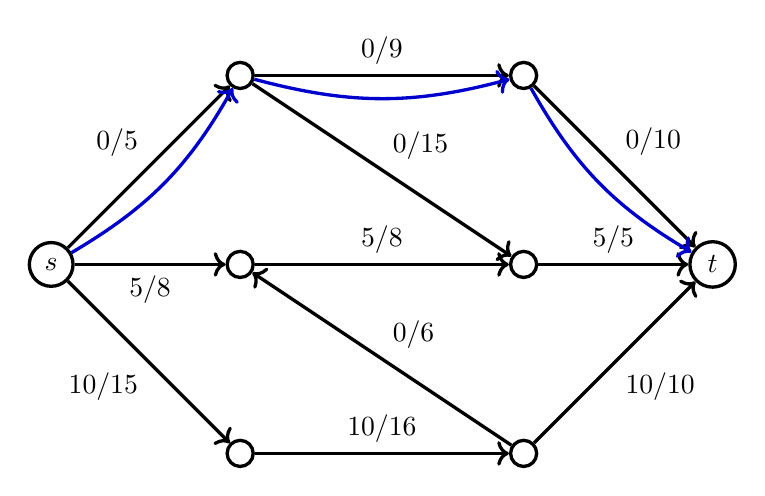
\begin{tikzpicture}[scale=1.2]
				\node[circle, draw, very thick] (0) at (0,0) {$s$};
				\node[circle, draw, very thick] (1) at (2,-2) {};
				\node[circle, draw, very thick] (2) at (2,0) {};
				\node[circle, draw, very thick] (3) at (2,2) {};
				\node[circle, draw, very thick] (4) at (5,-2) {};
				\node[circle, draw, very thick] (5) at (5,0) {};
				\node[circle, draw, very thick] (6) at (5,2) {};
				\node[circle, draw, very thick] (7) at (7,0) {$t$};
				
				\draw[very thick, ->]  (0) -- (1) node[midway,below left] () {$10/15$};
				\draw[very thick, ->]  (0) -- (2) node[midway,below] () {$5/8$};
				\draw[very thick, ->]  (0) -- (3) node[midway,above left] () {$0/5$};
				\draw[very thick, ->]  (1) -- (4) node[midway,above] () {$10/16$};
				\draw[very thick, ->]  (2) -- (5) node[midway,above] () {$5/8$};
				\draw[very thick, ->]  (3) -- (6) node[midway,above] () {$0/9$};
				\draw[very thick, ->]  (3) -- (5) node[midway,above right] () {$0/15$};
				\draw[very thick, ->]  (4) -- (2) node[midway,above right] () {$0/6$};
				\draw[very thick, ->]  (4) -- (7) node[midway,below right] () {$10/10$};
				\draw[very thick, ->]  (5) -- (7) node[midway,above] () {$5/5$};
				\draw[very thick, ->]  (6) -- (7) node[midway,above right] () {$0/10$};
				
				\draw[very thick, blue!80!black, ->] (0) to [bend right=15] (3);
				\draw[very thick, blue!80!black, ->] (3) to [bend right=15] (6);
				\draw[very thick, blue!80!black, ->] (6) to [bend right=15] (7);
			\end{tikzpicture}
		\end{center}
	\end{frame}
	
	\begin{frame}[plain]{Example}
		\begin{center}
			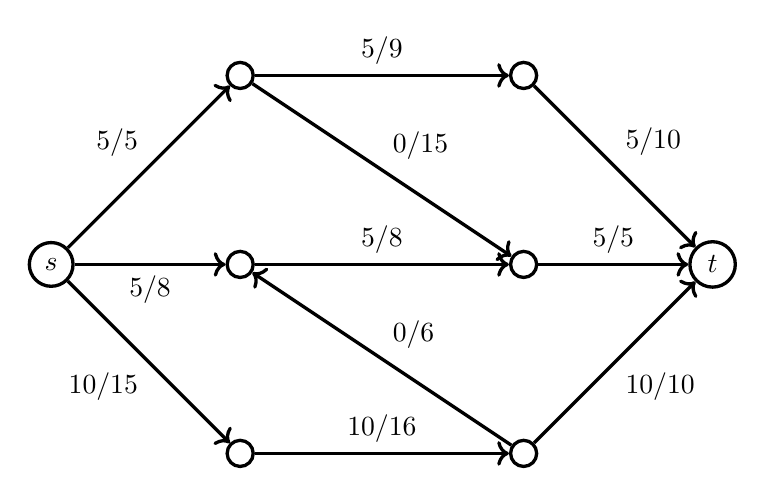
\begin{tikzpicture}[scale=1.2]
				\node[circle, draw, very thick] (0) at (0,0) {$s$};
				\node[circle, draw, very thick] (1) at (2,-2) {};
				\node[circle, draw, very thick] (2) at (2,0) {};
				\node[circle, draw, very thick] (3) at (2,2) {};
				\node[circle, draw, very thick] (4) at (5,-2) {};
				\node[circle, draw, very thick] (5) at (5,0) {};
				\node[circle, draw, very thick] (6) at (5,2) {};
				\node[circle, draw, very thick] (7) at (7,0) {$t$};
				
				\draw[very thick, ->]  (0) -- (1) node[midway,below left] () {$10/15$};
				\draw[very thick, ->]  (0) -- (2) node[midway,below] () {$5/8$};
				\draw[very thick, ->]  (0) -- (3) node[midway,above left] () {$5/5$};
				\draw[very thick, ->]  (1) -- (4) node[midway,above] () {$10/16$};
				\draw[very thick, ->]  (2) -- (5) node[midway,above] () {$5/8$};
				\draw[very thick, ->]  (3) -- (6) node[midway,above] () {$5/9$};
				\draw[very thick, ->]  (3) -- (5) node[midway,above right] () {$0/15$};
				\draw[very thick, ->]  (4) -- (2) node[midway,above right] () {$0/6$};
				\draw[very thick, ->]  (4) -- (7) node[midway,below right] () {$10/10$};
				\draw[very thick, ->]  (5) -- (7) node[midway,above] () {$5/5$};
				\draw[very thick, ->]  (6) -- (7) node[midway,above right] () {$5/10$};
			\end{tikzpicture}
		\end{center}
	\end{frame}
	
	\begin{frame}[plain]{Example}
		\begin{center}
			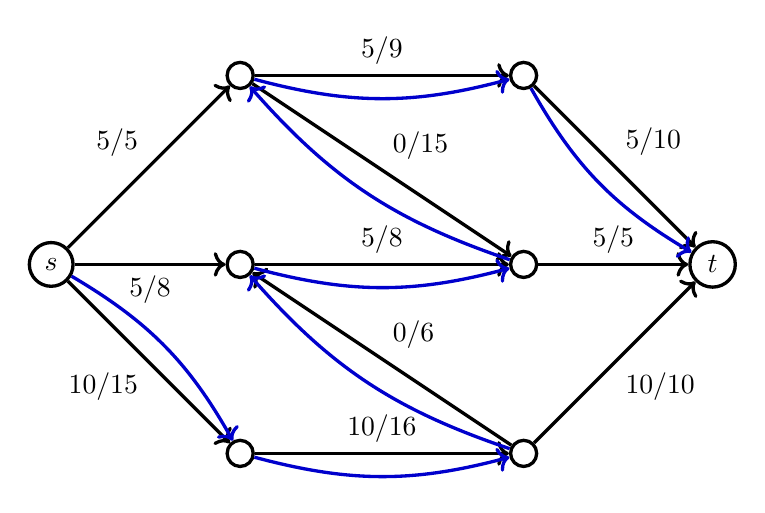
\begin{tikzpicture}[scale=1.2]
				\node[circle, draw, very thick] (0) at (0,0) {$s$};
				\node[circle, draw, very thick] (1) at (2,-2) {};
				\node[circle, draw, very thick] (2) at (2,0) {};
				\node[circle, draw, very thick] (3) at (2,2) {};
				\node[circle, draw, very thick] (4) at (5,-2) {};
				\node[circle, draw, very thick] (5) at (5,0) {};
				\node[circle, draw, very thick] (6) at (5,2) {};
				\node[circle, draw, very thick] (7) at (7,0) {$t$};
				
				\draw[very thick, ->]  (0) -- (1) node[midway,below left] () {$10/15$};
				\draw[very thick, ->]  (0) -- (2) node[midway,below] () {$5/8$};
				\draw[very thick, ->]  (0) -- (3) node[midway,above left] () {$5/5$};
				\draw[very thick, ->]  (1) -- (4) node[midway,above] () {$10/16$};
				\draw[very thick, ->]  (2) -- (5) node[midway,above] () {$5/8$};
				\draw[very thick, ->]  (3) -- (6) node[midway,above] () {$5/9$};
				\draw[very thick, ->]  (3) -- (5) node[midway,above right] () {$0/15$};
				\draw[very thick, ->]  (4) -- (2) node[midway,above right] () {$0/6$};
				\draw[very thick, ->]  (4) -- (7) node[midway,below right] () {$10/10$};
				\draw[very thick, ->]  (5) -- (7) node[midway,above] () {$5/5$};
				\draw[very thick, ->]  (6) -- (7) node[midway,above right] () {$5/10$};
				
				\draw[very thick, blue!80!black, ->] (0) to [bend left=15] (1);
				\draw[very thick, blue!80!black, ->] (1) to [bend right=15] (4);
				\draw[very thick, blue!80!black, ->] (4) to [bend left=15] (2);
				\draw[very thick, blue!80!black, ->] (2) to [bend right=15] (5);
				\draw[very thick, blue!80!black, ->] (5) to [bend left=15] (3);
				\draw[very thick, blue!80!black, ->] (3) to [bend right=15] (6);
				\draw[very thick, blue!80!black, ->] (6) to [bend right=15] (7);
			\end{tikzpicture}
		\end{center}
	\end{frame}
	
	\begin{frame}[plain]{Example}
		\begin{center}
			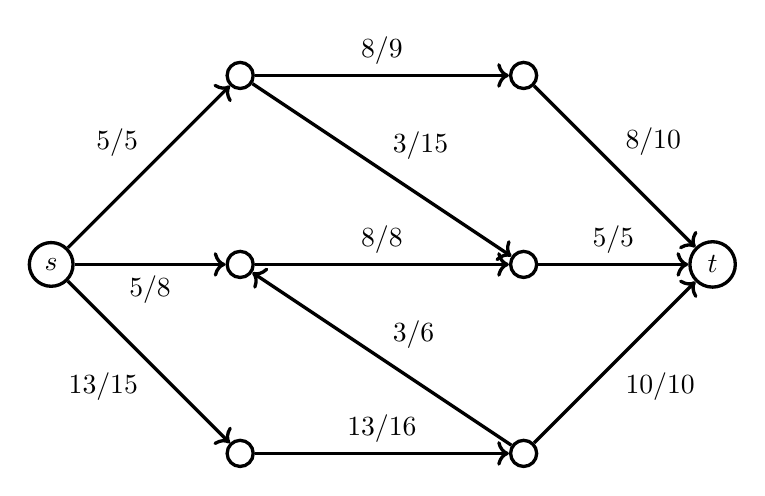
\begin{tikzpicture}[scale=1.2]
				\node[circle, draw, very thick] (0) at (0,0) {$s$};
				\node[circle, draw, very thick] (1) at (2,-2) {};
				\node[circle, draw, very thick] (2) at (2,0) {};
				\node[circle, draw, very thick] (3) at (2,2) {};
				\node[circle, draw, very thick] (4) at (5,-2) {};
				\node[circle, draw, very thick] (5) at (5,0) {};
				\node[circle, draw, very thick] (6) at (5,2) {};
				\node[circle, draw, very thick] (7) at (7,0) {$t$};
				
				\draw[very thick, ->]  (0) -- (1) node[midway,below left] () {$13/15$};
				\draw[very thick, ->]  (0) -- (2) node[midway,below] () {$5/8$};
				\draw[very thick, ->]  (0) -- (3) node[midway,above left] () {$5/5$};
				\draw[very thick, ->]  (1) -- (4) node[midway,above] () {$13/16$};
				\draw[very thick, ->]  (2) -- (5) node[midway,above] () {$8/8$};
				\draw[very thick, ->]  (3) -- (6) node[midway,above] () {$8/9$};
				\draw[very thick, ->]  (3) -- (5) node[midway,above right] () {$3/15$};
				\draw[very thick, ->]  (4) -- (2) node[midway,above right] () {$3/6$};
				\draw[very thick, ->]  (4) -- (7) node[midway,below right] () {$10/10$};
				\draw[very thick, ->]  (5) -- (7) node[midway,above] () {$5/5$};
				\draw[very thick, ->]  (6) -- (7) node[midway,above right] () {$8/10$};
			\end{tikzpicture}
		\end{center}
	\end{frame}
	
	\begin{frame}[plain]{Min-cut}
		\begin{itemize}
			\item We see that the value of the flow above is 23, but how do we know that's the maximum?
			\item The crux of showing that you can't do better is to look at the min-cut.
			\item This is a dual problem, asking what's the cheapest (minimum total capacity) set of vertices you need to cut to disconnect $s$ from $t$?
		\end{itemize}
	\end{frame}
	
	\begin{frame}[plain]{Example}
		\begin{center}
			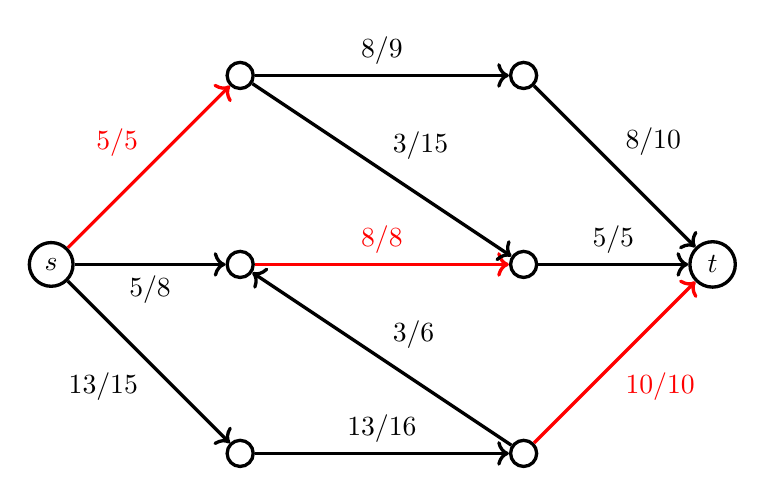
\begin{tikzpicture}[scale=1.2]
				\node[circle, draw, very thick] (0) at (0,0) {$s$};
				\node[circle, draw, very thick] (1) at (2,-2) {};
				\node[circle, draw, very thick] (2) at (2,0) {};
				\node[circle, draw, very thick] (3) at (2,2) {};
				\node[circle, draw, very thick] (4) at (5,-2) {};
				\node[circle, draw, very thick] (5) at (5,0) {};
				\node[circle, draw, very thick] (6) at (5,2) {};
				\node[circle, draw, very thick] (7) at (7,0) {$t$};
				
				\draw[very thick, ->]  (0) -- (1) node[midway,below left] () {$13/15$};
				\draw[very thick, ->]  (0) -- (2) node[midway,below] () {$5/8$};
				\draw[very thick, ->, red]  (0) -- (3) node[midway,above left] () {$5/5$};
				\draw[very thick, ->]  (1) -- (4) node[midway,above] () {$13/16$};
				\draw[very thick, ->, red]  (2) -- (5) node[midway,above] () {$8/8$};
				\draw[very thick, ->]  (3) -- (6) node[midway,above] () {$8/9$};
				\draw[very thick, ->]  (3) -- (5) node[midway,above right] () {$3/15$};
				\draw[very thick, ->]  (4) -- (2) node[midway,above right] () {$3/6$};
				\draw[very thick, ->, red]  (4) -- (7) node[midway,below right] () {$10/10$};
				\draw[very thick, ->]  (5) -- (7) node[midway,above] () {$5/5$};
				\draw[very thick, ->]  (6) -- (7) node[midway,above right] () {$8/10$};
			\end{tikzpicture}
		\end{center}
	\end{frame}
	
	\begin{frame}[plain]{Max-flow Min-cut}
		\begin{itemize}
			\item The fact that the min cut has value $23$ as well is no coincidence.
			\item It is not too hard to see that a max flow can never exceed a cut, as the flow has to pass from one side to the other of the cut using only the edges in the cut.
			\item So all cuts have costs greater or equal to the values of all flows.
			\item So if we find a flow that has value equal to the cost of a cut, that flow must be maximal and that cut minimal.
			\item The fact is, this is always the case. The maximum flow value is always equal to the cost of the minimum cut, proved by Ford and Fulkerson in 1962.
		\end{itemize}
	\end{frame}
	
	\begin{frame}[plain]{Max-flow Min-cut}
		\begin{itemize}
			\item The proof is not so hard, it is just a proof by looking at the greedy algorithm above and showing that if the flow is not yet equal to the cost of a minimum cut there must be some path that gets us closer.
			\item The proof also gives us that our greedy method always gets us closer to the answer in each step.
			\item But our algorithm is missing something to get all the way there!
		\end{itemize}
	\end{frame}
	
	\begin{frame}[plain]{Example}
		\begin{center}
			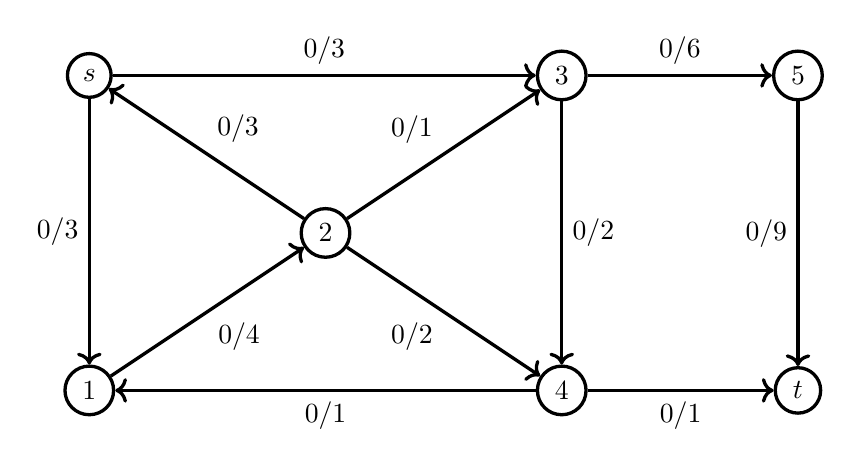
\begin{tikzpicture}
				\node[circle, draw, very thick] (A) at (0,0) {$s$};
				\node[circle, draw, very thick] (B) at (0,-4) {$1$};
				\node[circle, draw, very thick] (C) at (3,-2) {$2$};
				\node[circle, draw, very thick] (D) at (6,0) {$3$};
				\node[circle, draw, very thick] (E) at (6,-4) {$4$};
				\node[circle, draw, very thick] (F) at (9,0) {$5$};
				\node[circle, draw, very thick] (G) at (9,-4) {$t$};
				
				\draw[very thick, ->]  (A) -- (B) node[midway,left] () {$0/3$};
				\draw[very thick, ->]  (A) -- (D) node[midway,above] () {$0/3$};
				\draw[very thick, ->]  (B) -- (C) node[midway,below right] () {$0/4$};
				\draw[very thick, ->]  (C) -- (A) node[midway,above right] () {$0/3$};
				\draw[very thick, ->]  (C) -- (D) node[midway,above left] () {$0/1$};
				\draw[very thick, ->]  (C) -- (E) node[midway,below left] () {$0/2$};
				\draw[very thick, ->]  (D) -- (E) node[midway,right] () {$0/2$};
				\draw[very thick, ->]  (D) -- (F) node[midway,above] () {$0/6$};
				\draw[very thick, ->]  (E) -- (B) node[midway,below] () {$0/1$};
				\draw[very thick, ->]  (E) -- (G) node[midway,below] () {$0/1$};
				\draw[very thick, ->]  (F) -- (G) node[midway,left] () {$0/9$};
			\end{tikzpicture}
		\end{center}
	\end{frame}
	
	\begin{frame}[plain]{Example}
		\begin{center}
			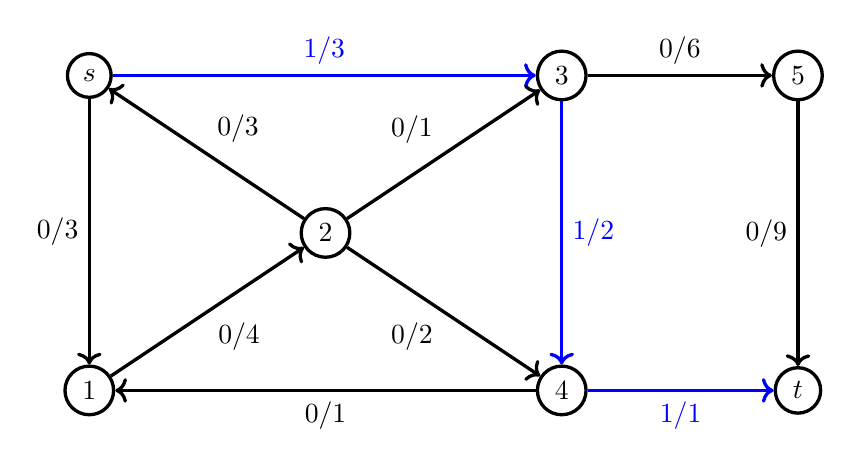
\begin{tikzpicture}
				\node[circle, draw, very thick] (A) at (0,0) {$s$};
				\node[circle, draw, very thick] (B) at (0,-4) {$1$};
				\node[circle, draw, very thick] (C) at (3,-2) {$2$};
				\node[circle, draw, very thick] (D) at (6,0) {$3$};
				\node[circle, draw, very thick] (E) at (6,-4) {$4$};
				\node[circle, draw, very thick] (F) at (9,0) {$5$};
				\node[circle, draw, very thick] (G) at (9,-4) {$t$};
				
				\draw[very thick, ->]  (A) -- (B) node[midway,left] () {$0/3$};
				\draw[very thick, ->, blue]  (A) -- (D) node[midway,above] () {$1/3$};
				\draw[very thick, ->]  (B) -- (C) node[midway,below right] () {$0/4$};
				\draw[very thick, ->]  (C) -- (A) node[midway,above right] () {$0/3$};
				\draw[very thick, ->]  (C) -- (D) node[midway,above left] () {$0/1$};
				\draw[very thick, ->]  (C) -- (E) node[midway,below left] () {$0/2$};
				\draw[very thick, ->, blue]  (D) -- (E) node[midway,right] () {$1/2$};
				\draw[very thick, ->]  (D) -- (F) node[midway,above] () {$0/6$};
				\draw[very thick, ->]  (E) -- (B) node[midway,below] () {$0/1$};
				\draw[very thick, ->, blue]  (E) -- (G) node[midway,below] () {$1/1$};
				\draw[very thick, ->]  (F) -- (G) node[midway,left] () {$0/9$};
			\end{tikzpicture}
		\end{center}
	\end{frame}
	
	\begin{frame}[plain]{Example}
		\begin{center}
			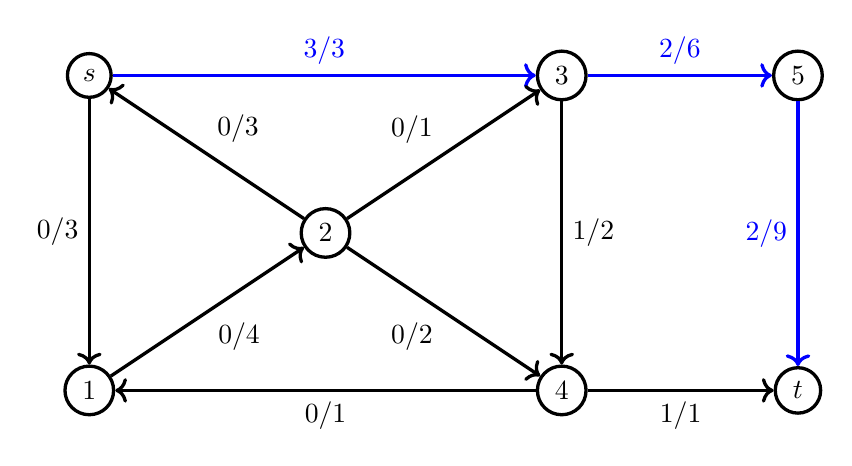
\begin{tikzpicture}
				\node[circle, draw, very thick] (A) at (0,0) {$s$};
				\node[circle, draw, very thick] (B) at (0,-4) {$1$};
				\node[circle, draw, very thick] (C) at (3,-2) {$2$};
				\node[circle, draw, very thick] (D) at (6,0) {$3$};
				\node[circle, draw, very thick] (E) at (6,-4) {$4$};
				\node[circle, draw, very thick] (F) at (9,0) {$5$};
				\node[circle, draw, very thick] (G) at (9,-4) {$t$};
				
				\draw[very thick, ->]  (A) -- (B) node[midway,left] () {$0/3$};
				\draw[very thick, ->, blue]  (A) -- (D) node[midway,above] () {$3/3$};
				\draw[very thick, ->]  (B) -- (C) node[midway,below right] () {$0/4$};
				\draw[very thick, ->]  (C) -- (A) node[midway,above right] () {$0/3$};
				\draw[very thick, ->]  (C) -- (D) node[midway,above left] () {$0/1$};
				\draw[very thick, ->]  (C) -- (E) node[midway,below left] () {$0/2$};
				\draw[very thick, ->]  (D) -- (E) node[midway,right] () {$1/2$};
				\draw[very thick, ->, blue]  (D) -- (F) node[midway,above] () {$2/6$};
				\draw[very thick, ->]  (E) -- (B) node[midway,below] () {$0/1$};
				\draw[very thick, ->]  (E) -- (G) node[midway,below] () {$1/1$};
				\draw[very thick, ->, blue]  (F) -- (G) node[midway,left] () {$2/9$};
			\end{tikzpicture}
		\end{center}
	\end{frame}
	
	\begin{frame}[plain]{Example}
		\begin{center}
			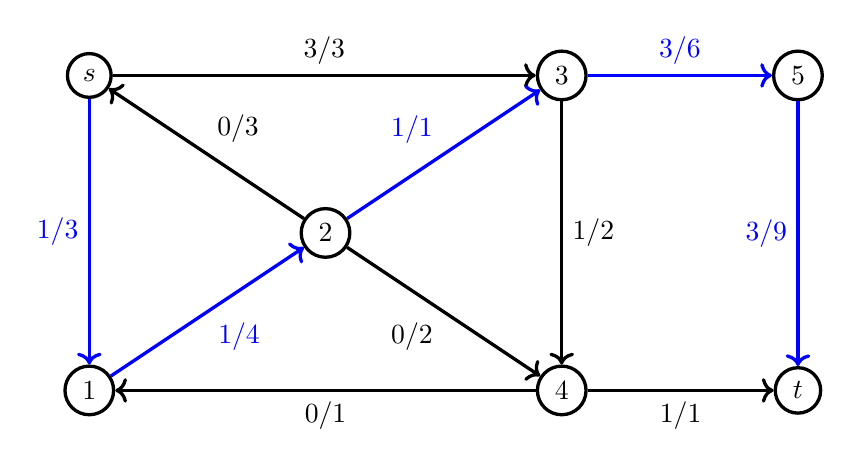
\begin{tikzpicture}
				\node[circle, draw, very thick] (A) at (0,0) {$s$};
				\node[circle, draw, very thick] (B) at (0,-4) {$1$};
				\node[circle, draw, very thick] (C) at (3,-2) {$2$};
				\node[circle, draw, very thick] (D) at (6,0) {$3$};
				\node[circle, draw, very thick] (E) at (6,-4) {$4$};
				\node[circle, draw, very thick] (F) at (9,0) {$5$};
				\node[circle, draw, very thick] (G) at (9,-4) {$t$};
				
				\draw[very thick, ->, blue]  (A) -- (B) node[midway,left] () {$1/3$};
				\draw[very thick, ->]  (A) -- (D) node[midway,above] () {$3/3$};
				\draw[very thick, ->, blue]  (B) -- (C) node[midway,below right] () {$1/4$};
				\draw[very thick, ->]  (C) -- (A) node[midway,above right] () {$0/3$};
				\draw[very thick, ->, blue]  (C) -- (D) node[midway,above left] () {$1/1$};
				\draw[very thick, ->]  (C) -- (E) node[midway,below left] () {$0/2$};
				\draw[very thick, ->]  (D) -- (E) node[midway,right] () {$1/2$};
				\draw[very thick, ->, blue]  (D) -- (F) node[midway,above] () {$3/6$};
				\draw[very thick, ->]  (E) -- (B) node[midway,below] () {$0/1$};
				\draw[very thick, ->]  (E) -- (G) node[midway,below] () {$1/1$};
				\draw[very thick, ->, blue]  (F) -- (G) node[midway,left] () {$3/9$};
			\end{tikzpicture}
		\end{center}
	\end{frame}
	
	\begin{frame}[plain]{Example}
		\begin{center}
			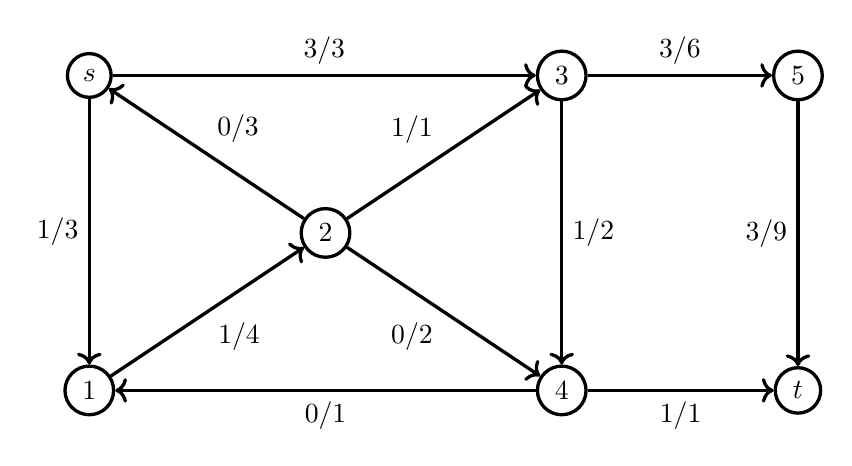
\begin{tikzpicture}
				\node[circle, draw, very thick] (A) at (0,0) {$s$};
				\node[circle, draw, very thick] (B) at (0,-4) {$1$};
				\node[circle, draw, very thick] (C) at (3,-2) {$2$};
				\node[circle, draw, very thick] (D) at (6,0) {$3$};
				\node[circle, draw, very thick] (E) at (6,-4) {$4$};
				\node[circle, draw, very thick] (F) at (9,0) {$5$};
				\node[circle, draw, very thick] (G) at (9,-4) {$t$};
				
				\draw[very thick, ->]  (A) -- (B) node[midway,left] () {$1/3$};
				\draw[very thick, ->]  (A) -- (D) node[midway,above] () {$3/3$};
				\draw[very thick, ->]  (B) -- (C) node[midway,below right] () {$1/4$};
				\draw[very thick, ->]  (C) -- (A) node[midway,above right] () {$0/3$};
				\draw[very thick, ->]  (C) -- (D) node[midway,above left] () {$1/1$};
				\draw[very thick, ->]  (C) -- (E) node[midway,below left] () {$0/2$};
				\draw[very thick, ->]  (D) -- (E) node[midway,right] () {$1/2$};
				\draw[very thick, ->]  (D) -- (F) node[midway,above] () {$3/6$};
				\draw[very thick, ->]  (E) -- (B) node[midway,below] () {$0/1$};
				\draw[very thick, ->]  (E) -- (G) node[midway,below] () {$1/1$};
				\draw[very thick, ->]  (F) -- (G) node[midway,left] () {$3/9$};
			\end{tikzpicture}
		\end{center}
	\end{frame}
	
	\begin{frame}[plain]{Now what?}
		\begin{itemize}
			\item We're stuck! The max flow is not $4$, and there is no max cut.
			\item But there is no way from $s$ to $t$ without using a full edge!
			\item What to do?
			\item<2-> What if we can "borrow" flow that's already been assigned?
			\item<2-> Then we can assign some more.
		\end{itemize}
	\end{frame}
	
	\begin{frame}[plain]{Example}
		\begin{center}
			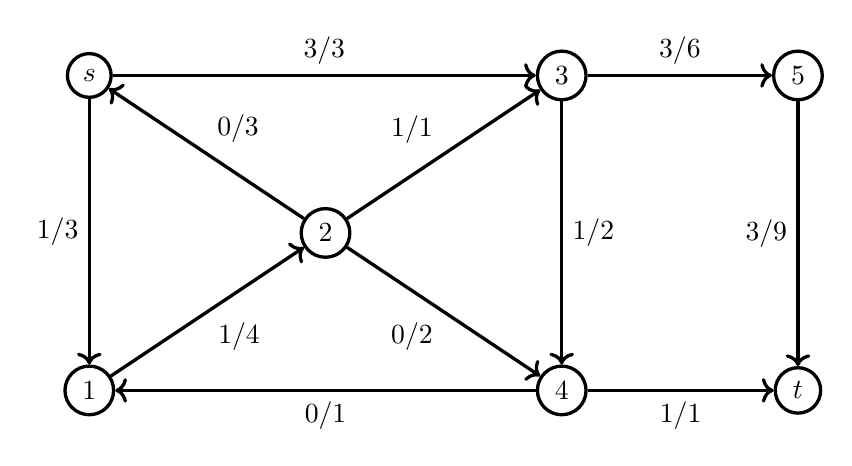
\begin{tikzpicture}
				\node[circle, draw, very thick] (A) at (0,0) {$s$};
				\node[circle, draw, very thick] (B) at (0,-4) {$1$};
				\node[circle, draw, very thick] (C) at (3,-2) {$2$};
				\node[circle, draw, very thick] (D) at (6,0) {$3$};
				\node[circle, draw, very thick] (E) at (6,-4) {$4$};
				\node[circle, draw, very thick] (F) at (9,0) {$5$};
				\node[circle, draw, very thick] (G) at (9,-4) {$t$};
				
				\draw[very thick, ->]  (A) -- (B) node[midway,left] () {$1/3$};
				\draw[very thick, ->]  (A) -- (D) node[midway,above] () {$3/3$};
				\draw[very thick, ->]  (B) -- (C) node[midway,below right] () {$1/4$};
				\draw[very thick, ->]  (C) -- (A) node[midway,above right] () {$0/3$};
				\draw[very thick, ->]  (C) -- (D) node[midway,above left] () {$1/1$};
				\draw[very thick, ->]  (C) -- (E) node[midway,below left] () {$0/2$};
				\draw[very thick, ->]  (D) -- (E) node[midway,right] () {$1/2$};
				\draw[very thick, ->]  (D) -- (F) node[midway,above] () {$3/6$};
				\draw[very thick, ->]  (E) -- (B) node[midway,below] () {$0/1$};
				\draw[very thick, ->]  (E) -- (G) node[midway,below] () {$1/1$};
				\draw[very thick, ->]  (F) -- (G) node[midway,left] () {$3/9$};
			\end{tikzpicture}
		\end{center}
	\end{frame}
	
	\begin{frame}[plain]{Example}
		\begin{center}
			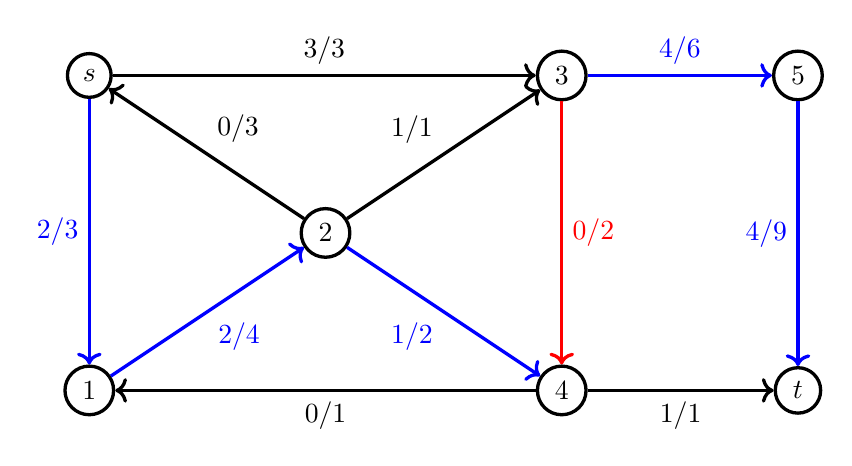
\begin{tikzpicture}
				\node[circle, draw, very thick] (A) at (0,0) {$s$};
				\node[circle, draw, very thick] (B) at (0,-4) {$1$};
				\node[circle, draw, very thick] (C) at (3,-2) {$2$};
				\node[circle, draw, very thick] (D) at (6,0) {$3$};
				\node[circle, draw, very thick] (E) at (6,-4) {$4$};
				\node[circle, draw, very thick] (F) at (9,0) {$5$};
				\node[circle, draw, very thick] (G) at (9,-4) {$t$};
				
				\draw[very thick, ->, blue]  (A) -- (B) node[midway,left] () {$2/3$};
				\draw[very thick, ->]  (A) -- (D) node[midway,above] () {$3/3$};
				\draw[very thick, ->, blue]  (B) -- (C) node[midway,below right] () {$2/4$};
				\draw[very thick, ->]  (C) -- (A) node[midway,above right] () {$0/3$};
				\draw[very thick, ->]  (C) -- (D) node[midway,above left] () {$1/1$};
				\draw[very thick, ->, blue]  (C) -- (E) node[midway,below left] () {$1/2$};
				\draw[very thick, ->, red]  (D) -- (E) node[midway,right] () {$0/2$};
				\draw[very thick, ->, blue]  (D) -- (F) node[midway,above] () {$4/6$};
				\draw[very thick, ->]  (E) -- (B) node[midway,below] () {$0/1$};
				\draw[very thick, ->]  (E) -- (G) node[midway,below] () {$1/1$};
				\draw[very thick, ->, blue]  (F) -- (G) node[midway,left] () {$4/9$};
			\end{tikzpicture}
		\end{center}
	\end{frame}
	
	\begin{frame}[plain]{Reverse edges}
		\begin{itemize}
			\item "Stealing" flow from an edge and following it backwards maintains all conditions we need.
			\item To program this the easiest way is just to add a backwards edge everywhere.
			\item If we add flow to a forward edge we subtract it from the backward edge, and vice versa.
			\item It can be proven that with this addition the algorithm always finds a max flow (try to think why).
		\end{itemize}
	\end{frame}
	
	\begin{frame}[plain]{Integers}
		\begin{itemize}
			\item Note that since our algorithm always increases the flow as much as it can along the path we choose, this means our flow will always have integer flow values if our capacities have integer values.
			\item If we do not have integer values, the greedy algorithm might not terminate!
		\end{itemize}
	\end{frame}
	
	\begin{frame}[plain]{Ford Fulkerson}
		\begin{itemize}
			\item This is known as the Ford-Fulkerson algorithm. So how fast is it if we have integer capacities?
			\item We have to find an augmenting path, we can do this using some standard graph search.
			\item<2-> So we have $\mathcal{O}(V + E)$ but the flow might just increase by one each time.
			\item<2-> Therefore the complexity is $\mathcal{O}(F(V + E))$ where $F$ is the maximum flow.
		\end{itemize}
	\end{frame}
	
	\begin{frame}[plain]{Edmond Karp}
		\begin{itemize}
			\item The problem is that if the capacities are very large, this is quite slow (in the worst case).
			\item There are ways around this, we just have to be more specific about how we find our augmenting paths.
			\item We essentially have two options, DFS and BFS:
			\item If you try both, you will see that BFS gives better worst-case behaviour.
		\end{itemize}
	\end{frame}
	
	\begin{frame}[plain]{Edmond Karp}
		\begin{itemize}
			\item Ford-Fulkerson with BFS is known as Edmond-Karp.
			\item The key feature one can prove is that if you saturate an edge several in the process, it must always be further away from the source along the augmenting path than last time. (Proof by contradiction, bit tricky, but not terrible)
			\item Then each edge can be saturated at most $V$ times, so we do at most $VE$ augmentations.
			\item Thus the time complexity is $\mathcal{O}(VE^2)$ at most (still also at most $\mathcal{O}(FE)$)
		\end{itemize}
	\end{frame}
	
	\begin{frame}[plain, fragile]{Implementation, part 1}
		\begin{scriptsize}
\begin{minted}{python}
# We use this as the queue module is not what we want
# It is meant for asynchronous tasks, not this
from collections import deque
from math import inf
# We define a class that takes in a graph
# and provides a max flow method
class FlowNetwork:
\end{minted}
\end{scriptsize}
\end{frame}
\begin{frame}[plain, fragile]{Implementation, part 2}
\begin{scriptsize}
\begin{minted}{python}
    def __init__(self, graph):
        # We construct the residual graph
        self.residual = [[] for _ in range(len(graph))]
        self.edges = []
        for vertex in range(len(graph)):
            for cap, neighbour in graph[vertex]:
                # Each edge is doubled and always adjacent
                # This means we can get the reverse edge with
                # ^1, since 0 and 1 map to each other, 2 and 3
                # and so on (just flips last bit in number)
                # Before adding the edge the length of the list
                # gives the index the new edge will be at
                self.residual[vertex].append(len(self.edges))
                # Initially we have a budget of up to 'cap'
                e1 = [vertex, neighbour, cap]
                self.edges.append(e1)
                self.residual[neighbour].append(len(self.edges))
                # But the reverse edge has no initial budget
                e2 = [neighbour, vertex, 0]
                self.edges.append(e2)
\end{minted}
\end{scriptsize}
\end{frame}
\begin{frame}[plain, fragile]{Implementation, part 3}
\begin{scriptsize}
\begin{minted}{python}
    def bfs(self, s, t, parent): # s is the source, t the sink
        # Keep an array of the flow found, augmenting path pushes to vertex
        flow = [0 for i in range(len(self.residual))]
        # Initialize BFS
        queue = deque()
        queue.append(s)
        flow[s] = inf
        while queue:
            cur = queue.popleft()
            for index in self.residual[cur]:
                edge = self.edges[index]
                # edge[1] is endpoint of edge, edge[2] is cap
                # So if we've already looked at endpoint or
                # the edge is saturated we skip
                if flow[edge[1]] > 0 or edge[2] == 0:
                    continue
                # Otherwise update and continue
                queue.append(edge[1])
                flow[edge[1]] = min(flow[cur], edge[2])
                parent[edge[1]] = index
        # flow[t] contains how much we can push to sink
        return flow[t]
\end{minted}
\end{scriptsize}
\end{frame}
\begin{frame}[plain, fragile]{Implementation, part 4}
\begin{scriptsize}
\begin{minted}{python}
    def max_flow(self, s, t):
        parent = [-1 for _ in range(len(self.residual))]
        max_flow = 0
        # This will set path_flow to the result of bfs
        # and only loop if that is > 0
        while path_flow := self.bfs(s, t, parent):
            # Add it to max flow
            max_flow += path_flow
            # Now we need to walk along the path
            # and update the residual capacities
            position = t
            while position != s:
                index = parent[position]
                # Decrease residual capacity
                self.edges[index][2] -= path_flow
                # The reverse edge is adjacent, ^1 trick
                self.edges[index ^ 1][2] += path_flow
                position = self.edges[index][0]
         # And we're done!
        return max_flow
\end{minted}
		\end{scriptsize}
	\end{frame}
	
	\begin{frame}[plain]{But then what?}
		\begin{itemize}
			\item What do we do with this then?
			\item In fact very many things can be modeled as maximum flow.
			\item Probably one of the most practical algorithms in this course. But to show some examples, first we have to look at a general construction that allows us to have multiple sources and multiple sinks.
			\item Any suggestions how?
		\end{itemize}
	\end{frame}
	
	\begin{frame}[plain]{Multi source/sink}
	\begin{center}
		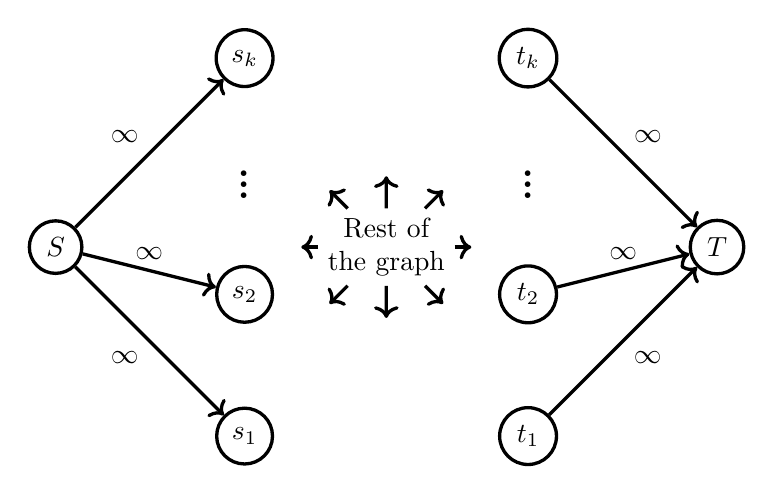
\begin{tikzpicture}[scale=1.2]
			\node[circle, draw, very thick] (0) at (0,0) {$S$};
			\node[circle, draw, very thick] (1) at (2,-2) {$s_1$};
			\node[circle, draw, very thick] (2) at (2,-0.5) {$s_2$};
			\node (3) at (2,0.75) {\Huge $\vdots$};
			\node[circle, draw, very thick] (4) at (2,2) {$s_k$};
			\node[align=center] (5) at (3.5,0) {Rest of \\ the graph};
			\node[circle, draw, very thick] (6) at (5,-2) {$t_1$};
			\node[circle, draw, very thick] (7) at (5,-0.5) {$t_2$};
			\node (8) at (5,0.75) {\Huge $\vdots$};
			\node[circle, draw, very thick] (9) at (5,2) {$t_k$};
			\node[circle, draw, very thick] (A) at (7,0) {$T$};
			
			
			\draw[very thick, ->]  (0) -- (1) node[midway,below left] () {$\infty$};
			\draw[very thick, ->]  (0) -- (2) node[midway,above] () {$\infty$};
			\draw[very thick, ->]  (0) -- (4) node[midway,above left] () {$\infty$};
			
			\draw[very thick, ->]  (6) -- (A) node[midway,below right] () {$\infty$};
			\draw[very thick, ->]  (7) -- (A) node[midway,above] () {$\infty$};
			\draw[very thick, ->]  (9) -- (A) node[midway,above right] () {$\infty$};
			
			\draw[very thick, ->] (5) -- ++(0,0.75);
			\draw[very thick, ->] (5) -- ++(0.6,0.6);
			\draw[very thick, ->] (5) -- ++(0.9,0);
			\draw[very thick, ->] (5) -- ++(0.6,-0.6);
			\draw[very thick, ->] (5) -- ++(0,-0.75);
			\draw[very thick, ->] (5) -- ++(-0.6,-0.6);
			\draw[very thick, ->] (5) -- ++(-0.9,0);
			\draw[very thick, ->] (5) -- ++(-0.6,0.6);
		\end{tikzpicture}
	\end{center}
	\end{frame}
	
	\begin{frame}[plain]{Bipartite matching}
		\begin{itemize}
			\item There are many practical situations where we want to pair up some set of objects with another, but not every pair is acceptable, and each objects can only be in one pair.
			\item As an example my team solved a problem for a contest of practical problems hosted by Google (Hash Code) about pairing employees to tasks they can handle using a variant of this method.
			\item We can use maximum flow just by making the graph on the last slide (except with 1 instead of $\infty$ so each vertex can only be in ine pair) and putting an edge with capacity $1$ between any two vertices we are allowed to pair together.
		\end{itemize}
	\end{frame}
	
	\begin{frame}[plain]{Bipartite matching}
		\begin{center}
			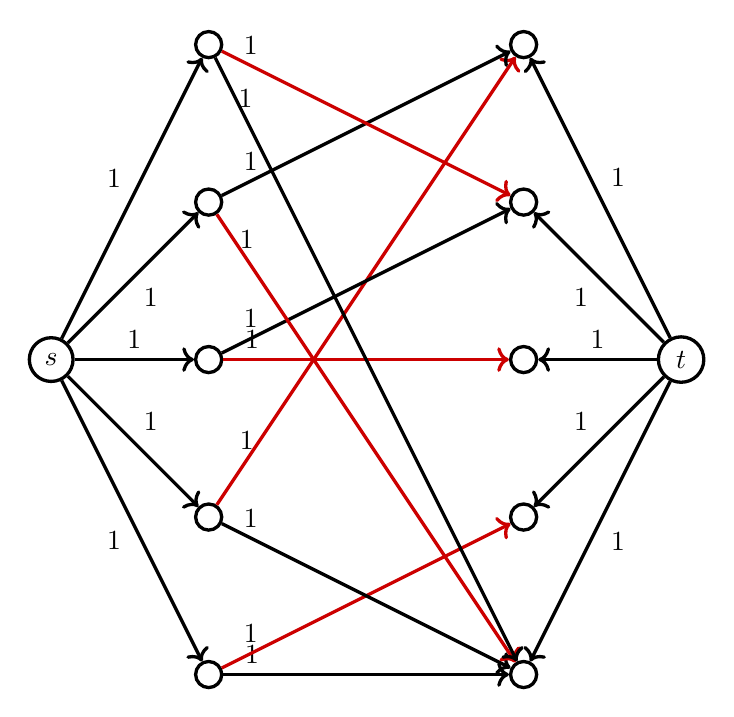
\begin{tikzpicture}[scale=1]
				\node[circle, draw, very thick] (0) at (0,0) {$s$};
				\node[circle, draw, very thick] (1) at (2,-4) {};
				\node[circle, draw, very thick] (2) at (2,-2) {};
				\node[circle, draw, very thick] (3) at (2,0) {};
				\node[circle, draw, very thick] (4) at (2,2) {};
				\node[circle, draw, very thick] (5) at (2,4) {};
				\node[circle, draw, very thick] (6) at (6,-4) {};
				\node[circle, draw, very thick] (7) at (6,-2) {};
				\node[circle, draw, very thick] (8) at (6,0) {};
				\node[circle, draw, very thick] (9) at (6,2) {};
				\node[circle, draw, very thick] (A) at (6,4) {};
				\node[circle, draw, very thick] (B) at (8,0) {$t$};
				
				\def\pp{0.1} 
				
				\draw[very thick, ->] (1) -- (6) node[pos=\pp,above] () {$1$};
				\draw[very thick, ->, red!80!black] (1) -- (7) node[pos=\pp,above] () {\color{black} $1$};
				\draw[very thick, ->] (2) -- (6) node[pos=\pp,above] () {$1$};
				\draw[very thick, ->, red!80!black] (2) -- (A) node[pos=\pp,above] () {\color{black} $1$};
				\draw[very thick, ->, red!80!black] (3) -- (8) node[pos=\pp,above] () {\color{black}$1$};
				\draw[very thick, ->] (3) -- (9) node[pos=\pp,above] () {$1$};
				\draw[very thick, ->, red!80!black] (4) -- (6) node[pos=\pp,above] () {\color{black} $1$};
				\draw[very thick, ->] (4) -- (A) node[pos=\pp,above] () {$1$};
				\draw[very thick, ->] (5) -- (6) node[pos=\pp,above] () {$1$};
				\draw[very thick, ->, red!80!black] (5) -- (9) node[pos=\pp,above] () {\color{black} $1$};
				
				\draw[very thick, ->]  (0) -- (1) node[midway,below left] () {$1$};
				\draw[very thick, ->]  (0) -- (2) node[midway,above right] () {$1$};
				\draw[very thick, ->]  (0) -- (3) node[midway,above] () {$1$};
				\draw[very thick, ->]  (0) -- (4) node[midway,below right] () {$1$};
				\draw[very thick, ->]  (0) -- (5) node[midway,above left] () {$1$};
				
				\draw[very thick, ->]  (B) -- (6) node[midway,below right] () {$1$};
				\draw[very thick, ->]  (B) -- (7) node[midway,above left] () {$1$};
				\draw[very thick, ->]  (B) -- (8) node[midway,above] () {$1$};
				\draw[very thick, ->]  (B) -- (9) node[midway,below left] () {$1$};
				\draw[very thick, ->]  (B) -- (A) node[midway,above right] () {$1$};
			\end{tikzpicture}
		\end{center}
	\end{frame}
	
	\begin{frame}[plain]{Bipartite matching}
		\begin{itemize}
			\item Here actually the "bad" bound of $\mathcal{O}(FE)$ is better than $\mathcal{O}(VE^2)$ as $FE$ simplifies to $VE$ in this graph.
			\item Though we will see later a way to do it in $\mathcal{O}(E\sqrt{V})$.
			\item We will also later consider the case where each pairing has different weights, like the cost of hiring an employee to do a particular task, where we want to minimise total cost as well.
			\item Let's first take two other examples of problems solvable with max flow.
		\end{itemize}
	\end{frame}
	
	\begin{frame}[plain]{Baseball league}
		\begin{itemize}
			\item Let's consider an example from baseball.
			\item During a league a fixed schedule of games will be played, whichever teams has strictly the most wins at the end is the winner (let's just say for ties there are no winners).
			\item At some point in the league you wonder, can your favourite team $x$ win the league?
		\end{itemize}
	\end{frame}
	
	\begin{frame}[plain]{Baseball league}
		\begin{itemize}
			\item Clearly it's best for team $x$ to win all remaining games, so let's assume that's the case.
			\item Then we need to choose a winner for all other games such that no team gets as many wins as team $x$ has in this hypothetical full win scenario.
			\item This is an assignment problem of games to winners, so we can model it with maximum flow.
			\item Each game (or rather pairing of teams) gets a node which can flow to winners, and the winners have a limit of flow to the sink based on how many wins would put them ahead of $x$.
			\item Then we just check if this graph has a saturating flow!
		\end{itemize}
	\end{frame}
	
	\begin{frame}[plain]{Baseball league}
	\begin{center}
		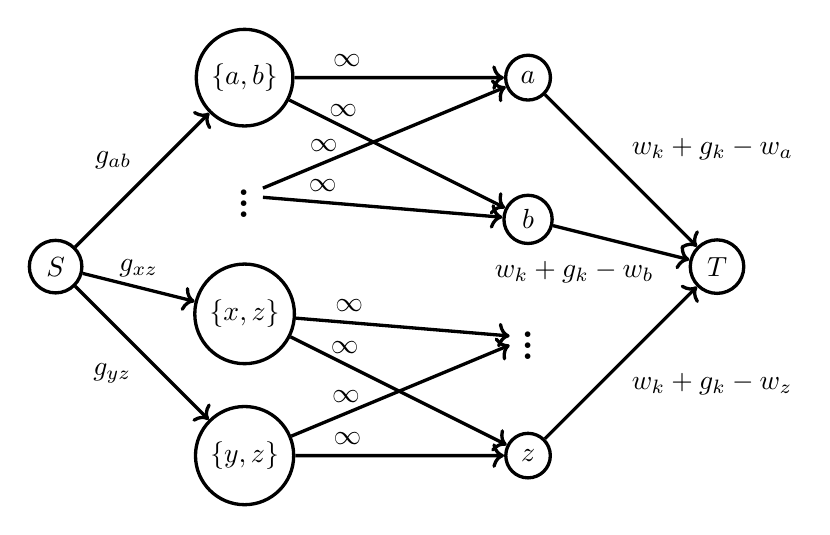
\begin{tikzpicture}[scale=1.2]
			\node[circle, draw, very thick] (0) at (0,0) {$S$};
			\node[circle, draw, very thick] (1) at (2,-2) {$\{y, z\}$};
			\node[circle, draw, very thick] (2) at (2,-0.5) {$\{x, z\}$};
			\node (3) at (2,0.75) {\Huge $\vdots$};
			\node[circle, draw, very thick] (4) at (2,2) {$\{a, b\}$};
			\node[circle, draw, very thick] (6) at (5,-2) {$z$};
			\node (8) at (5,-0.75) {\Huge $\vdots$};
			\node[circle, draw, very thick] (7) at (5,0.5) {$b$};
			\node[circle, draw, very thick] (9) at (5,2) {$a$};
			\node[circle, draw, very thick] (A) at (7,0) {$T$};
			
			\def\pp{0.25} 
			
			\draw[very thick, ->]  (0) -- (1) node[midway,below left] () {$g_{yz}$};
			\draw[very thick, ->]  (0) -- (2) node[midway,above] () {$g_{xz}$};
			\draw[very thick, ->]  (0) -- (4) node[midway,above left] () {$g_{ab}$};
			
			\draw[very thick, ->]  (6) -- (A) node[midway,below right] () {$w_k + g_k - w_z$};
			\draw[very thick, ->]  (7) -- (A) node[midway,below left = 0.1 and -0.55] () {$w_k + g_k - w_b$};
			\draw[very thick, ->]  (9) -- (A) node[midway,above right] () {$w_k + g_k - w_a$};
			
			\draw[very thick, ->] (4) -- (9) node[pos=\pp, above] {$\infty$};
			\draw[very thick, ->] (4) -- (7) node[pos=\pp, above] {$\infty$};
			
			\draw[very thick, ->] (3) -- (9) node[pos=\pp, above] {$\infty$};
			\draw[very thick, ->] (3) -- (7) node[pos=\pp, above] {$\infty$};
			
			\draw[very thick, ->] (2) -- (8) node[pos=\pp, above] {$\infty$};
			\draw[very thick, ->] (2) -- (6) node[pos=\pp, above] {$\infty$};
			
			\draw[very thick, ->] (1) -- (8) node[pos=\pp, above] {$\infty$};
			\draw[very thick, ->] (1) -- (6) node[pos=\pp, above] {$\infty$};
			
		\end{tikzpicture}
	\end{center}
	\end{frame}
	
	\begin{frame}[plain]{Theorems}
		\begin{itemize}
			\item Some theorems also give us use cases for maximum flow. König's theorem for example gives us the solution to the minimum vertex cover (fewest vertices needed to touch every edge) problem in bipartite graphs in terms of the maximum matching. 
			\item Menger's theorem tells us that the number of disjoint paths between $s$ and $t$ in a graph is equal to the maximum flow from $s$ to $t$ if every edge has unit capacity. This way we can find whether a graph is $k$-edge-connected. (There is also a version of Menger's theorem for vertex connectivity)
		\end{itemize}
	\end{frame}
	
	\begin{frame}[plain]{Tricks}
		\begin{itemize}
			\item Aside from there being many theorems that show that max flow or problems solved solved by max flow are equivalent to something else, there are also many constructions that allow us to solve more general problems.
			\item We already saw how to have multiple sources and sinks, but let's look at some other examples of this.
			\item We'll look at vertex capacities and flows with demands as two examples.
		\end{itemize}
	\end{frame}
	
	\begin{frame}[plain]{Vertex split}
		\begin{itemize}
			\item Say we have a flow problem, but we want to limit the amount of flow that goes through each vertex as well
			\item We can split the vertex, and make it have an internal edge with a capacity
			\item So each edge pointing to $v$ goes to a new vertex $v_{\text{in}}$, each pointing out goes from a new vertex $v_{\text{out}}$, and then we put an edge from $v_{\text{in}}$ to $v_{\text{out}}$ with our desired capacity
		\end{itemize}
	\end{frame}
	
	\begin{frame}[plain]{Vertex split}
		\begin{itemize}
			\item Say we have a flow problem, but we want to limit the amount of flow that goes through each vertex as well
			\item We can split the vertex, and make it have an internal edge with a capacity
			\item So each edge pointing to $v$ goes to a new vertex $v_{\text{in}}$, each pointing out goes from a new vertex $v_{\text{out}}$, and then we put an edge from $v_{\text{in}}$ to $v_{\text{out}}$ with our desired capacity
		\end{itemize}
	\end{frame}
	
	\begin{frame}[plain]{With demands}
		\begin{itemize}
			\item What if we want each edge $e$ to have a minimum flow $d_e$? We can ask for any flow or even the minimum flow
			\item We can actually augment the graph to solve this with maximum flow as well
			\item This won't be in the homework, but is a good exercise for those wanting to try it
		\end{itemize}
	\end{frame}
	
	\begin{frame}[plain]{Capacity scaling}
		\begin{itemize}
			\item Another trick one can use to do max flow is to start with only capacities 0/1 and solve that in $\mathcal{O}(FE) = \mathcal{O}(E)$
			\item Then we double all the capacities and flows that should be $\geq 2$ and solve again, each edge needs to be incremented at most once,
			 so this takes $\mathcal{O}(E^2)$
			 \item Then we double, and repeat
			 \item This trick is known as capacity scaling, which solves max flow in $\mathcal{O}(E^2 \log(F))$
		\end{itemize}
	\end{frame}
	
	\begin{frame}[plain]{Dinic's algorithm}
		\begin{itemize}
			\item Edmond-Karp is the original polynomial algorithm for maximum-flow, but there are (many) others.
		\end{itemize}
		\only<1>{
		\begin{center}
			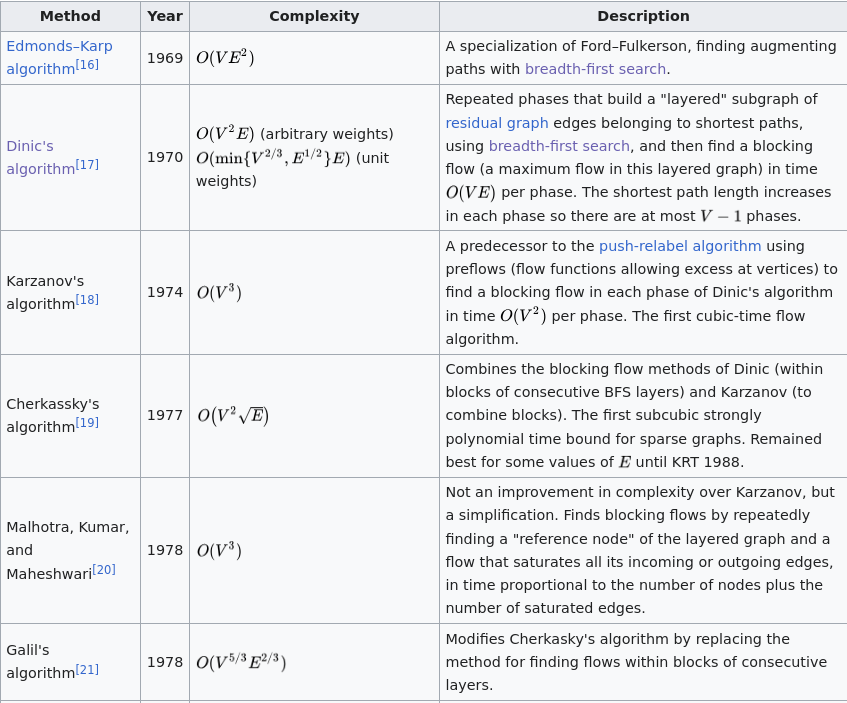
\includegraphics[scale=0.3]{tp1}
		\end{center}
		}
		\only<2>{
			\begin{center}
				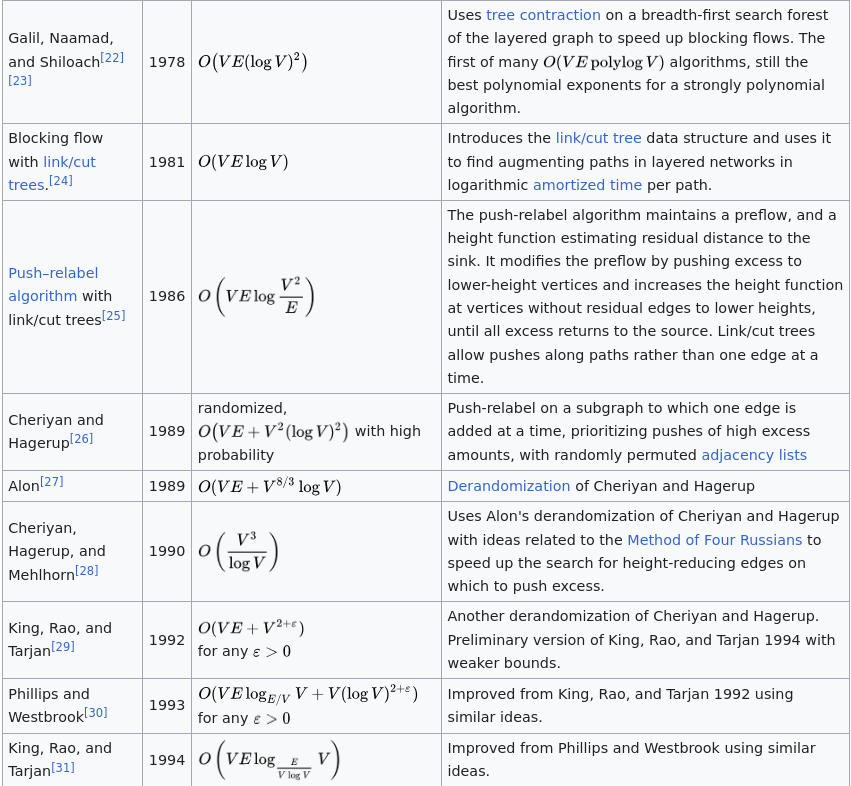
\includegraphics[scale=0.3]{tp2}
			\end{center}
		}
		\only<3>{
			\begin{center}
				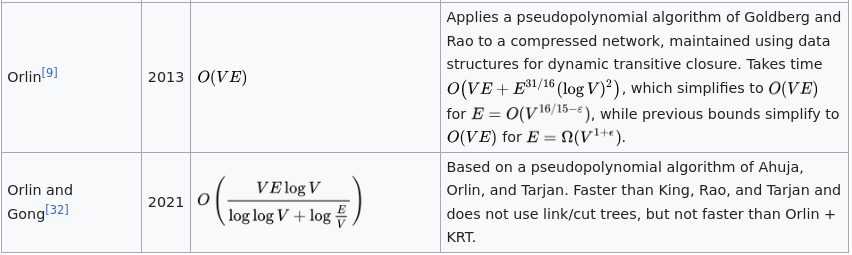
\includegraphics[scale=0.3]{tp3}
			\end{center}
		}
		\only<4>{
			\begin{center}
				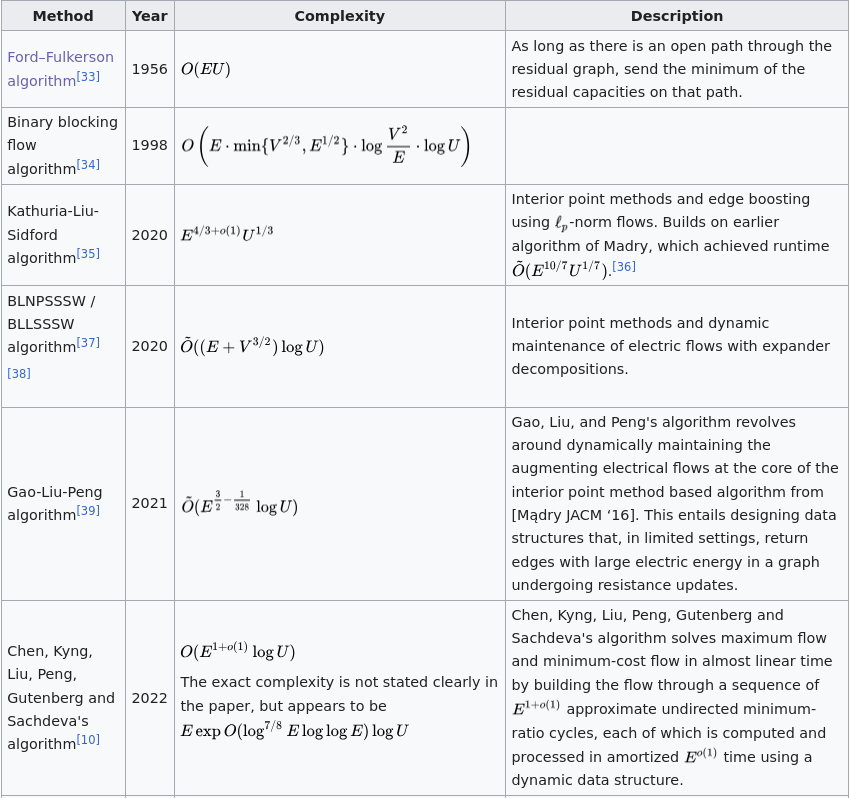
\includegraphics[scale=0.3]{tp4}
			\end{center}
		}
		\only<5>{
			\begin{center}
				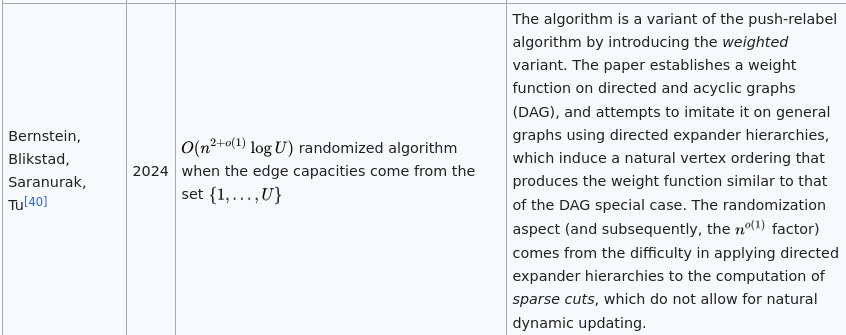
\includegraphics[scale=0.3]{tp5}
			\end{center}
		}
	\end{frame}
	
	\begin{frame}[plain]{Dinic's algorithm}
		\begin{itemize}
			\item Many of these are not that performant in practice as they don't start being faster until for unfeasibly large graphs.
			\item But there are two that are commonly implemented as performance improvements over Edmond-Karp.
			\item Those are Dinic's algorithm and the Push-Relabel algorithm.
			\item We will not look at Push-Relabel as it is quite technical, but I recommend it for interested students. 
			\item Instead we look at Dinic's algorithm.
		\end{itemize}
	\end{frame}
	
	\begin{frame}[plain]{Dinic's algorithm}
		\begin{itemize}
			\item We need two concepts. 
			\item A blocking flow is a flow such that every path from the sink to the source has at least one saturated edge (note this is not necessarily a maximal flow).
			\item A layered network of a graph $G$ is a graph constructed in the following manner:
			\begin{itemize}
				\item Let $L(v)$ be the length of the shortest (unweighted) path from the source to $v$ using only edges with capacity left.
				\item Construct a subgraph of $G$ keeping only the edges $u \rightarrow v$ such that $L(v) = L(u) + 1$.
			\end{itemize}
		\end{itemize}
	\end{frame}
	
	\begin{frame}[plain]{Dinic's algorithm}
		\begin{itemize}
			\item The algorithm proceeds by repeatedly constructing the layered network of our graph.
			\item Each time we find a blocking flow in that layered network and add it to our total flow.
			\item If we get no flow in the layered network we terminate.
			\item If we found no flow, then the layered network has no unsaturated path from $s$ to $t$ and then $G$ doesn't either, so the flow is already maximum.
		\end{itemize}
	\end{frame}
	
	\begin{frame}[plain]{Example}
		\begin{center}
			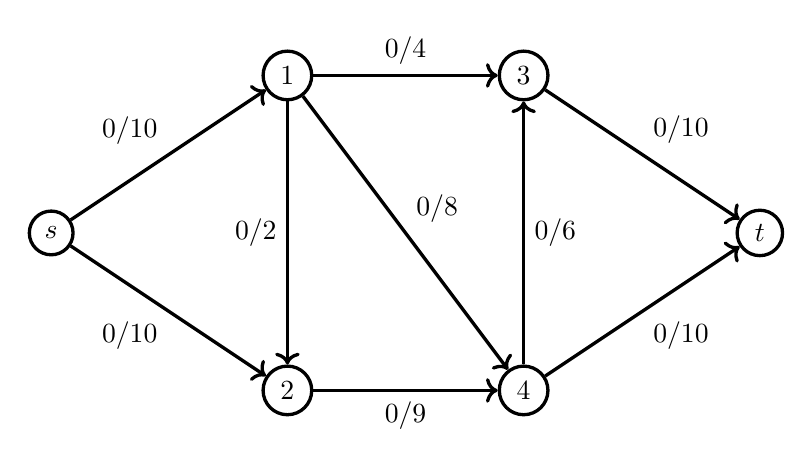
\begin{tikzpicture}
				\node[circle, draw, very thick] (S) at (0,0) {$s$};
				\node[circle, draw, very thick] (1) at (3,2) {$1$};
				\node[circle, draw, very thick] (2) at (3,-2) {$2$};
				\node[circle, draw, very thick] (3) at (6,2) {$3$};
				\node[circle, draw, very thick] (4) at (6,-2) {$4$};
				\node[circle, draw, very thick] (T) at (9,0) {$t$};
				
				\draw[very thick, ->]  (S) -- (1) node[midway,above left] () {$0/10$};
				\draw[very thick, ->]  (S) -- (2) node[midway,below left] () {$0/10$};
				\draw[very thick, ->]  (1) -- (2) node[midway,left] () {$0/2$};
				\draw[very thick, ->]  (1) -- (3) node[midway,above] () {$0/4$};
				\draw[very thick, ->]  (1) -- (4) node[midway,above right] () {$0/8$};
				\draw[very thick, ->]  (2) -- (4) node[midway,below] () {$0/9$};
				\draw[very thick, ->]  (3) -- (T) node[midway,above right] () {$0/10$};
				\draw[very thick, ->]  (4) -- (3) node[midway,right] () {$0/6$};
				\draw[very thick, ->]  (4) -- (T) node[midway,below right] () {$0/10$};
			\end{tikzpicture}
		\end{center}
	\end{frame}
	
	\begin{frame}[plain]{Example}
		\begin{center}
			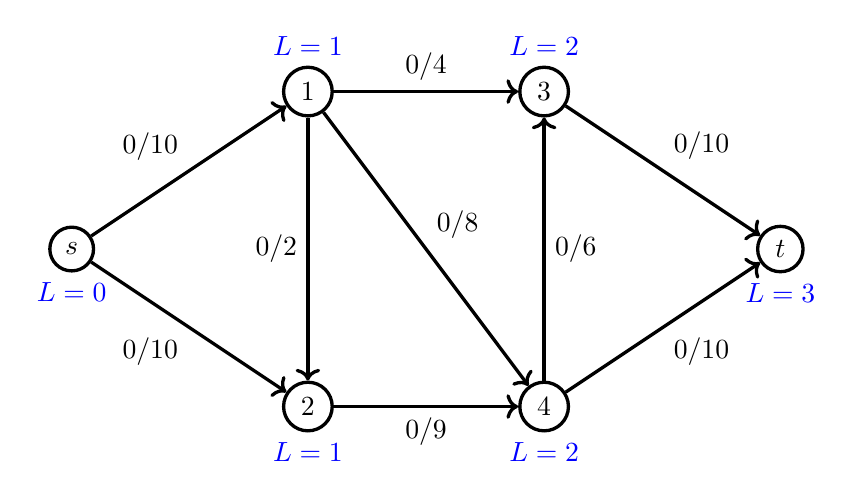
\begin{tikzpicture}
				\node[circle, draw, very thick] (S) at (0,0) {$s$};
				\node[circle, draw, very thick] (1) at (3,2) {$1$};
				\node[circle, draw, very thick] (2) at (3,-2) {$2$};
				\node[circle, draw, very thick] (3) at (6,2) {$3$};
				\node[circle, draw, very thick] (4) at (6,-2) {$4$};
				\node[circle, draw, very thick] (T) at (9,0) {$t$};
				
				\node [below=0cm of S, blue] {$L = 0$};
				\node [below=0cm of 2, blue] {$L = 1$};
				\node [below=0cm of 4, blue] {$L = 2$};
				\node [above=0cm of 1, blue] {$L = 1$};
				\node [above=0cm of 3, blue] {$L = 2$};
				\node [below=0cm of T, blue] {$L = 3$};
				
				\draw[very thick, ->]  (S) -- (1) node[midway,above left] () {$0/10$};
				\draw[very thick, ->]  (S) -- (2) node[midway,below left] () {$0/10$};
				\draw[very thick, ->]  (1) -- (2) node[midway,left] () {$0/2$};
				\draw[very thick, ->]  (1) -- (3) node[midway,above] () {$0/4$};
				\draw[very thick, ->]  (1) -- (4) node[midway,above right] () {$0/8$};
				\draw[very thick, ->]  (2) -- (4) node[midway,below] () {$0/9$};
				\draw[very thick, ->]  (3) -- (T) node[midway,above right] () {$0/10$};
				\draw[very thick, ->]  (4) -- (3) node[midway,right] () {$0/6$};
				\draw[very thick, ->]  (4) -- (T) node[midway,below right] () {$0/10$};
			\end{tikzpicture}
		\end{center}
	\end{frame}
	
	\begin{frame}[plain]{Example}
		\begin{center}
			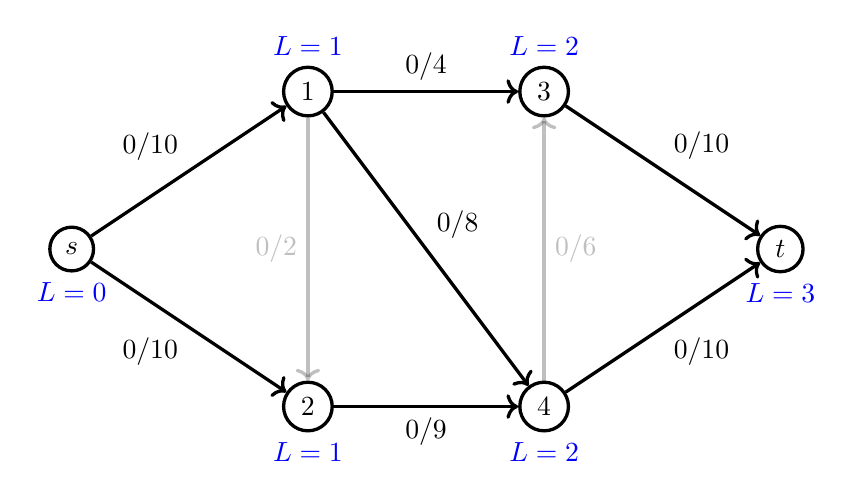
\begin{tikzpicture}
				\node[circle, draw, very thick] (S) at (0,0) {$s$};
				\node[circle, draw, very thick] (1) at (3,2) {$1$};
				\node[circle, draw, very thick] (2) at (3,-2) {$2$};
				\node[circle, draw, very thick] (3) at (6,2) {$3$};
				\node[circle, draw, very thick] (4) at (6,-2) {$4$};
				\node[circle, draw, very thick] (T) at (9,0) {$t$};
				
				\node [below=0cm of S, blue] {$L = 0$};
				\node [below=0cm of 2, blue] {$L = 1$};
				\node [below=0cm of 4, blue] {$L = 2$};
				\node [above=0cm of 1, blue] {$L = 1$};
				\node [above=0cm of 3, blue] {$L = 2$};
				\node [below=0cm of T, blue] {$L = 3$};
				
				\draw[very thick, ->]  (S) -- (1) node[midway,above left] () {$0/10$};
				\draw[very thick, ->]  (S) -- (2) node[midway,below left] () {$0/10$};
				\draw[very thick, ->, opacity=0.25]  (1) -- (2) node[midway,left] () {$0/2$};
				\draw[very thick, ->]  (1) -- (3) node[midway,above] () {$0/4$};
				\draw[very thick, ->]  (1) -- (4) node[midway,above right] () {$0/8$};
				\draw[very thick, ->]  (2) -- (4) node[midway,below] () {$0/9$};
				\draw[very thick, ->]  (3) -- (T) node[midway,above right] () {$0/10$};
				\draw[very thick, ->, opacity=0.25]  (4) -- (3) node[midway,right] () {$0/6$};
				\draw[very thick, ->]  (4) -- (T) node[midway,below right] () {$0/10$};
			\end{tikzpicture}
		\end{center}
	\end{frame}
	
	\begin{frame}[plain]{Example}
		\begin{center}
			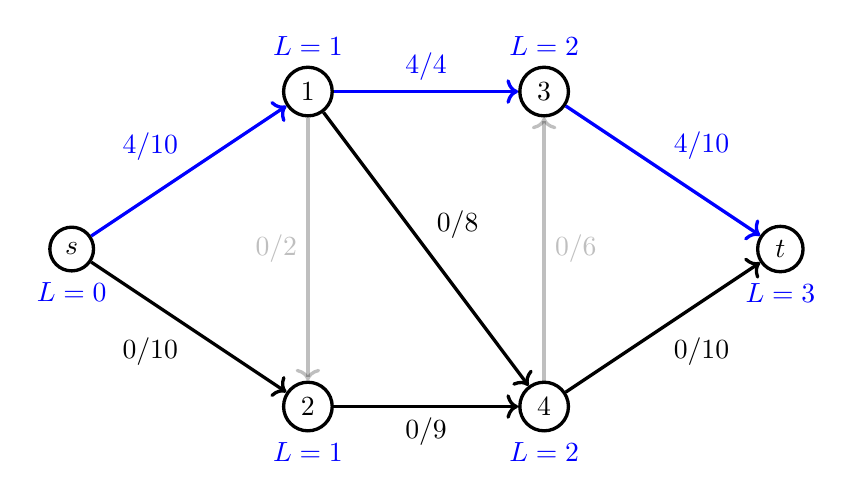
\begin{tikzpicture}
				\node[circle, draw, very thick] (S) at (0,0) {$s$};
				\node[circle, draw, very thick] (1) at (3,2) {$1$};
				\node[circle, draw, very thick] (2) at (3,-2) {$2$};
				\node[circle, draw, very thick] (3) at (6,2) {$3$};
				\node[circle, draw, very thick] (4) at (6,-2) {$4$};
				\node[circle, draw, very thick] (T) at (9,0) {$t$};
				
				\node [below=0cm of S, blue] {$L = 0$};
				\node [below=0cm of 2, blue] {$L = 1$};
				\node [below=0cm of 4, blue] {$L = 2$};
				\node [above=0cm of 1, blue] {$L = 1$};
				\node [above=0cm of 3, blue] {$L = 2$};
				\node [below=0cm of T, blue] {$L = 3$};
				
				\draw[very thick, ->, blue]  (S) -- (1) node[midway,above left] () {$4/10$};
				\draw[very thick, ->]  (S) -- (2) node[midway,below left] () {$0/10$};
				\draw[very thick, ->, opacity=0.25]  (1) -- (2) node[midway,left] () {$0/2$};
				\draw[very thick, ->, blue]  (1) -- (3) node[midway,above] () {$4/4$};
				\draw[very thick, ->]  (1) -- (4) node[midway,above right] () {$0/8$};
				\draw[very thick, ->]  (2) -- (4) node[midway,below] () {$0/9$};
				\draw[very thick, ->, blue]  (3) -- (T) node[midway,above right] () {$4/10$};
				\draw[very thick, ->, opacity=0.25]  (4) -- (3) node[midway,right] () {$0/6$};
				\draw[very thick, ->]  (4) -- (T) node[midway,below right] () {$0/10$};
			\end{tikzpicture}
		\end{center}
	\end{frame}
	
	\begin{frame}[plain]{Example}
		\begin{center}
			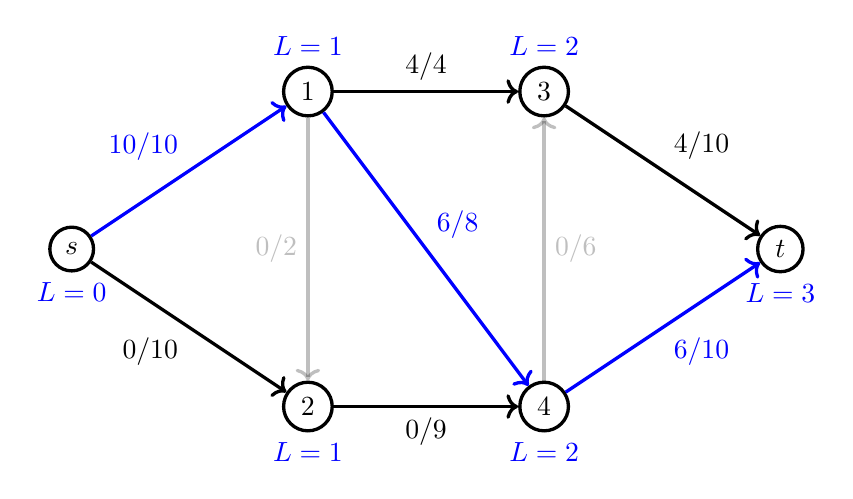
\begin{tikzpicture}
				\node[circle, draw, very thick] (S) at (0,0) {$s$};
				\node[circle, draw, very thick] (1) at (3,2) {$1$};
				\node[circle, draw, very thick] (2) at (3,-2) {$2$};
				\node[circle, draw, very thick] (3) at (6,2) {$3$};
				\node[circle, draw, very thick] (4) at (6,-2) {$4$};
				\node[circle, draw, very thick] (T) at (9,0) {$t$};
				
				\node [below=0cm of S, blue] {$L = 0$};
				\node [below=0cm of 2, blue] {$L = 1$};
				\node [below=0cm of 4, blue] {$L = 2$};
				\node [above=0cm of 1, blue] {$L = 1$};
				\node [above=0cm of 3, blue] {$L = 2$};
				\node [below=0cm of T, blue] {$L = 3$};
				
				\draw[very thick, ->, blue]  (S) -- (1) node[midway,above left] () {$10/10$};
				\draw[very thick, ->]  (S) -- (2) node[midway,below left] () {$0/10$};
				\draw[very thick, ->, opacity=0.25]  (1) -- (2) node[midway,left] () {$0/2$};
				\draw[very thick, ->]  (1) -- (3) node[midway,above] () {$4/4$};
				\draw[very thick, ->, blue]  (1) -- (4) node[midway,above right] () {$6/8$};
				\draw[very thick, ->]  (2) -- (4) node[midway,below] () {$0/9$};
				\draw[very thick, ->]  (3) -- (T) node[midway,above right] () {$4/10$};
				\draw[very thick, ->, opacity=0.25]  (4) -- (3) node[midway,right] () {$0/6$};
				\draw[very thick, ->, blue]  (4) -- (T) node[midway,below right] () {$6/10$};
			\end{tikzpicture}
		\end{center}
	\end{frame}
	
	\begin{frame}[plain]{Example}
		\begin{center}
			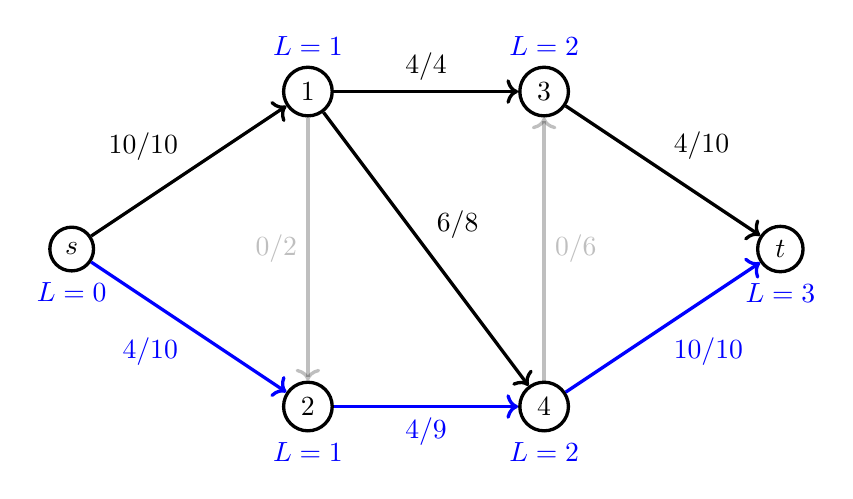
\begin{tikzpicture}
				\node[circle, draw, very thick] (S) at (0,0) {$s$};
				\node[circle, draw, very thick] (1) at (3,2) {$1$};
				\node[circle, draw, very thick] (2) at (3,-2) {$2$};
				\node[circle, draw, very thick] (3) at (6,2) {$3$};
				\node[circle, draw, very thick] (4) at (6,-2) {$4$};
				\node[circle, draw, very thick] (T) at (9,0) {$t$};
				
				\node [below=0cm of S, blue] {$L = 0$};
				\node [below=0cm of 2, blue] {$L = 1$};
				\node [below=0cm of 4, blue] {$L = 2$};
				\node [above=0cm of 1, blue] {$L = 1$};
				\node [above=0cm of 3, blue] {$L = 2$};
				\node [below=0cm of T, blue] {$L = 3$};
				
				\draw[very thick, ->]  (S) -- (1) node[midway,above left] () {$10/10$};
				\draw[very thick, ->, blue]  (S) -- (2) node[midway,below left] () {$4/10$};
				\draw[very thick, ->, opacity=0.25]  (1) -- (2) node[midway,left] () {$0/2$};
				\draw[very thick, ->]  (1) -- (3) node[midway,above] () {$4/4$};
				\draw[very thick, ->]  (1) -- (4) node[midway,above right] () {$6/8$};
				\draw[very thick, ->, blue]  (2) -- (4) node[midway,below] () {$4/9$};
				\draw[very thick, ->]  (3) -- (T) node[midway,above right] () {$4/10$};
				\draw[very thick, ->, opacity=0.25]  (4) -- (3) node[midway,right] () {$0/6$};
				\draw[very thick, ->, blue]  (4) -- (T) node[midway,below right] () {$10/10$};
			\end{tikzpicture}
		\end{center}
	\end{frame}
	
	\begin{frame}[plain]{Example}
		\begin{center}
			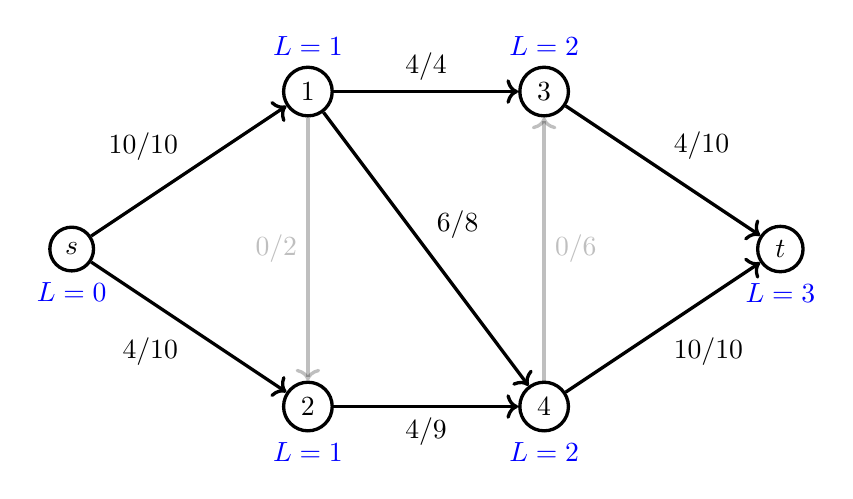
\begin{tikzpicture}
				\node[circle, draw, very thick] (S) at (0,0) {$s$};
				\node[circle, draw, very thick] (1) at (3,2) {$1$};
				\node[circle, draw, very thick] (2) at (3,-2) {$2$};
				\node[circle, draw, very thick] (3) at (6,2) {$3$};
				\node[circle, draw, very thick] (4) at (6,-2) {$4$};
				\node[circle, draw, very thick] (T) at (9,0) {$t$};
				
				\node [below=0cm of S, blue] {$L = 0$};
				\node [below=0cm of 2, blue] {$L = 1$};
				\node [below=0cm of 4, blue] {$L = 2$};
				\node [above=0cm of 1, blue] {$L = 1$};
				\node [above=0cm of 3, blue] {$L = 2$};
				\node [below=0cm of T, blue] {$L = 3$};
				
				\draw[very thick, ->]  (S) -- (1) node[midway,above left] () {$10/10$};
				\draw[very thick, ->]  (S) -- (2) node[midway,below left] () {$4/10$};
				\draw[very thick, ->, opacity=0.25]  (1) -- (2) node[midway,left] () {$0/2$};
				\draw[very thick, ->]  (1) -- (3) node[midway,above] () {$4/4$};
				\draw[very thick, ->]  (1) -- (4) node[midway,above right] () {$6/8$};
				\draw[very thick, ->]  (2) -- (4) node[midway,below] () {$4/9$};
				\draw[very thick, ->]  (3) -- (T) node[midway,above right] () {$4/10$};
				\draw[very thick, ->, opacity=0.25]  (4) -- (3) node[midway,right] () {$0/6$};
				\draw[very thick, ->]  (4) -- (T) node[midway,below right] () {$10/10$};
			\end{tikzpicture}
		\end{center}
	\end{frame}
	
	
	
	\begin{frame}[plain]{Example}
		\begin{center}
			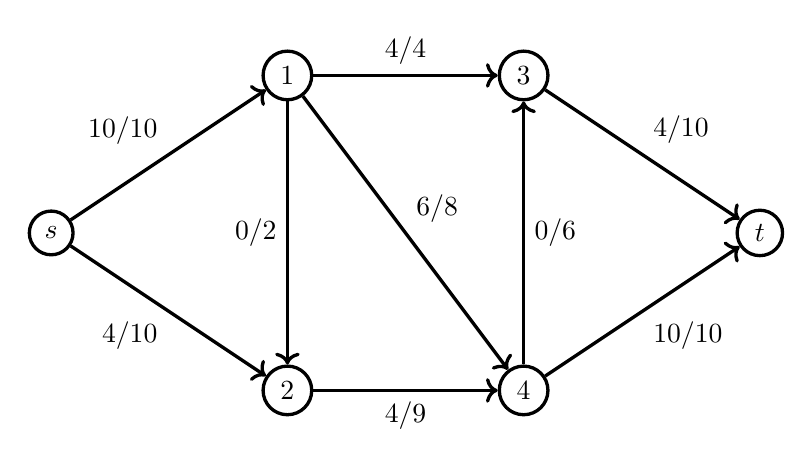
\begin{tikzpicture}
				\node[circle, draw, very thick] (S) at (0,0) {$s$};
				\node[circle, draw, very thick] (1) at (3,2) {$1$};
				\node[circle, draw, very thick] (2) at (3,-2) {$2$};
				\node[circle, draw, very thick] (3) at (6,2) {$3$};
				\node[circle, draw, very thick] (4) at (6,-2) {$4$};
				\node[circle, draw, very thick] (T) at (9,0) {$t$};
				
				\draw[very thick, ->]  (S) -- (1) node[midway,above left] () {$10/10$};
				\draw[very thick, ->]  (S) -- (2) node[midway,below left] () {$4/10$};
				\draw[very thick, ->]  (1) -- (2) node[midway,left] () {$0/2$};
				\draw[very thick, ->]  (1) -- (3) node[midway,above] () {$4/4$};
				\draw[very thick, ->]  (1) -- (4) node[midway,above right] () {$6/8$};
				\draw[very thick, ->]  (2) -- (4) node[midway,below] () {$4/9$};
				\draw[very thick, ->]  (3) -- (T) node[midway,above right] () {$4/10$};
				\draw[very thick, ->]  (4) -- (3) node[midway,right] () {$0/6$};
				\draw[very thick, ->]  (4) -- (T) node[midway,below right] () {$10/10$};
			\end{tikzpicture}
		\end{center}
	\end{frame}
	
	\begin{frame}[plain]{Example}
		\begin{center}
			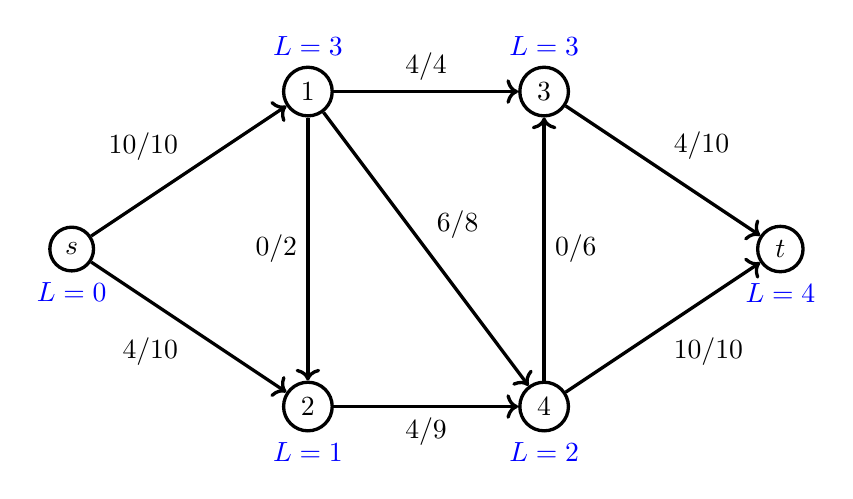
\begin{tikzpicture}
				\node[circle, draw, very thick] (S) at (0,0) {$s$};
				\node[circle, draw, very thick] (1) at (3,2) {$1$};
				\node[circle, draw, very thick] (2) at (3,-2) {$2$};
				\node[circle, draw, very thick] (3) at (6,2) {$3$};
				\node[circle, draw, very thick] (4) at (6,-2) {$4$};
				\node[circle, draw, very thick] (T) at (9,0) {$t$};
				
				\node [below=0cm of S, blue] {$L = 0$};
				\node [below=0cm of 2, blue] {$L = 1$};
				\node [below=0cm of 4, blue] {$L = 2$};
				\node [above=0cm of 1, blue] {$L = 3$};
				\node [above=0cm of 3, blue] {$L = 3$};
				\node [below=0cm of T, blue] {$L = 4$};
				
				\draw[very thick, ->]  (S) -- (1) node[midway,above left] () {$10/10$};
				\draw[very thick, ->]  (S) -- (2) node[midway,below left] () {$4/10$};
				\draw[very thick, ->]  (1) -- (2) node[midway,left] () {$0/2$};
				\draw[very thick, ->]  (1) -- (3) node[midway,above] () {$4/4$};
				\draw[very thick, ->]  (1) -- (4) node[midway,above right] () {$6/8$};
				\draw[very thick, ->]  (2) -- (4) node[midway,below] () {$4/9$};
				\draw[very thick, ->]  (3) -- (T) node[midway,above right] () {$4/10$};
				\draw[very thick, ->]  (4) -- (3) node[midway,right] () {$0/6$};
				\draw[very thick, ->]  (4) -- (T) node[midway,below right] () {$10/10$};
			\end{tikzpicture}
		\end{center}
	\end{frame}
	
	\begin{frame}[plain]{Example}
		\begin{center}
			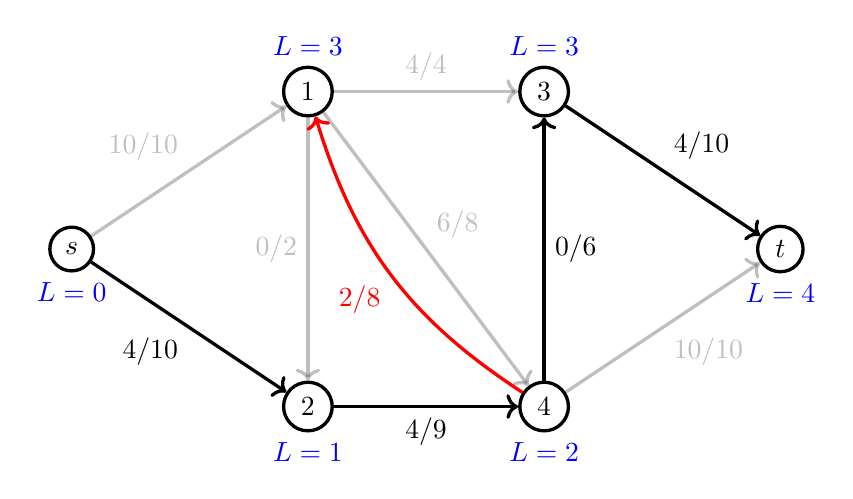
\begin{tikzpicture}
				\node[circle, draw, very thick] (S) at (0,0) {$s$};
				\node[circle, draw, very thick] (1) at (3,2) {$1$};
				\node[circle, draw, very thick] (2) at (3,-2) {$2$};
				\node[circle, draw, very thick] (3) at (6,2) {$3$};
				\node[circle, draw, very thick] (4) at (6,-2) {$4$};
				\node[circle, draw, very thick] (T) at (9,0) {$t$};
				
				\node [below=0cm of S, blue] {$L = 0$};
				\node [below=0cm of 2, blue] {$L = 1$};
				\node [below=0cm of 4, blue] {$L = 2$};
				\node [above=0cm of 1, blue] {$L = 3$};
				\node [above=0cm of 3, blue] {$L = 3$};
				\node [below=0cm of T, blue] {$L = 4$};
				
				\draw[very thick, ->, opacity=0.25]  (S) -- (1) node[midway,above left] () {$10/10$};
				\draw[very thick, ->]  (S) -- (2) node[midway,below left] () {$4/10$};
				\draw[very thick, ->, opacity=0.25]  (1) -- (2) node[midway,left] () {$0/2$};
				\draw[very thick, ->, opacity=0.25]  (1) -- (3) node[midway,above] () {$4/4$};
				\draw[very thick, ->, opacity=0.25]  (1) -- (4) node[midway,above right] () {$6/8$};
				\draw[very thick, ->, red]  (4) to[bend left=20] node[midway,below left] () {$2/8$} (1) ;
				\draw[very thick, ->]  (2) -- (4) node[midway,below] () {$4/9$};
				\draw[very thick, ->]  (3) -- (T) node[midway,above right] () {$4/10$};
				\draw[very thick, ->]  (4) -- (3) node[midway,right] () {$0/6$};
				\draw[very thick, ->, opacity=0.25]  (4) -- (T) node[midway,below right] () {$10/10$};
			\end{tikzpicture}
		\end{center}
	\end{frame}
	
	\begin{frame}[plain]{Example}
		\begin{center}
			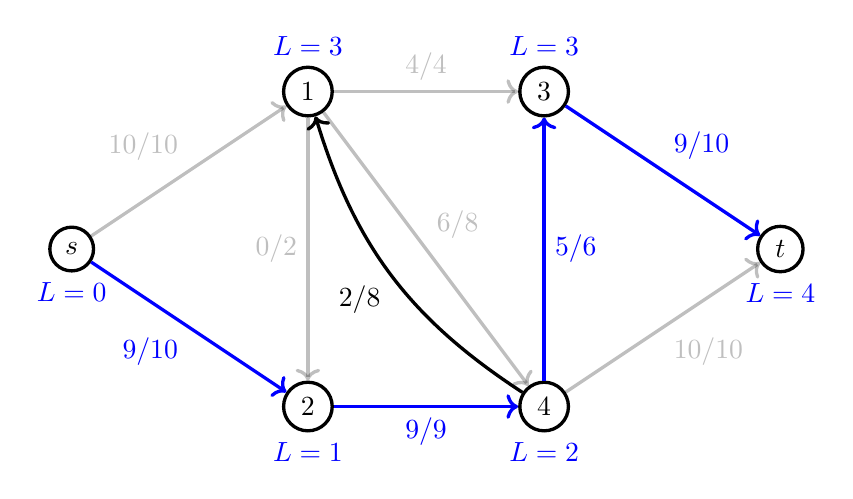
\begin{tikzpicture}
				\node[circle, draw, very thick] (S) at (0,0) {$s$};
				\node[circle, draw, very thick] (1) at (3,2) {$1$};
				\node[circle, draw, very thick] (2) at (3,-2) {$2$};
				\node[circle, draw, very thick] (3) at (6,2) {$3$};
				\node[circle, draw, very thick] (4) at (6,-2) {$4$};
				\node[circle, draw, very thick] (T) at (9,0) {$t$};
				
				\node [below=0cm of S, blue] {$L = 0$};
				\node [below=0cm of 2, blue] {$L = 1$};
				\node [below=0cm of 4, blue] {$L = 2$};
				\node [above=0cm of 1, blue] {$L = 3$};
				\node [above=0cm of 3, blue] {$L = 3$};
				\node [below=0cm of T, blue] {$L = 4$};
				
				\draw[very thick, ->, opacity=0.25]  (S) -- (1) node[midway,above left] () {$10/10$};
				\draw[very thick, ->, blue]  (S) -- (2) node[midway,below left] () {$9/10$};
				\draw[very thick, ->, opacity=0.25]  (1) -- (2) node[midway,left] () {$0/2$};
				\draw[very thick, ->, opacity=0.25]  (1) -- (3) node[midway,above] () {$4/4$};
				\draw[very thick, ->, opacity=0.25]  (1) -- (4) node[midway,above right] () {$6/8$};
				\draw[very thick, ->]  (4) to[bend left=20] node[midway,below left] () {$2/8$} (1) ;
				\draw[very thick, ->, blue]  (2) -- (4) node[midway,below] () {$9/9$};
				\draw[very thick, ->, blue]  (3) -- (T) node[midway,above right] () {$9/10$};
				\draw[very thick, ->, blue]  (4) -- (3) node[midway,right] () {$5/6$};
				\draw[very thick, ->, opacity=0.25]  (4) -- (T) node[midway,below right] () {$10/10$};
			\end{tikzpicture}
		\end{center}
	\end{frame}
	
	\begin{frame}[plain]{Example}
		\begin{center}
			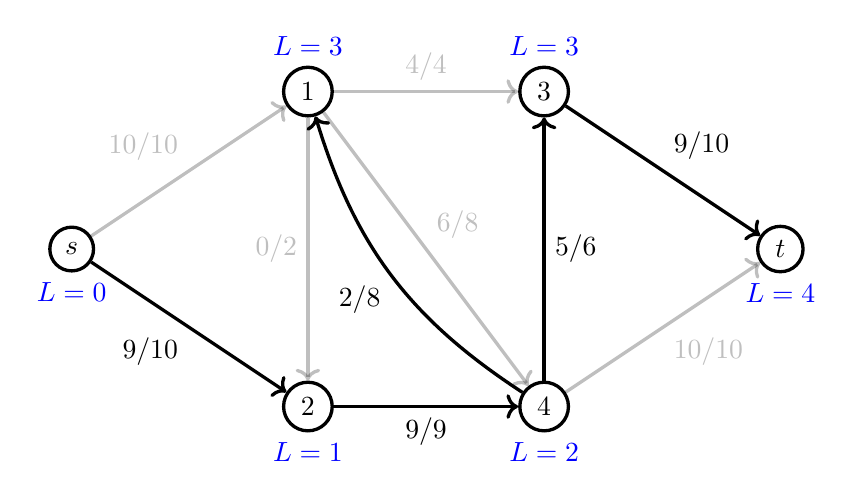
\begin{tikzpicture}
				\node[circle, draw, very thick] (S) at (0,0) {$s$};
				\node[circle, draw, very thick] (1) at (3,2) {$1$};
				\node[circle, draw, very thick] (2) at (3,-2) {$2$};
				\node[circle, draw, very thick] (3) at (6,2) {$3$};
				\node[circle, draw, very thick] (4) at (6,-2) {$4$};
				\node[circle, draw, very thick] (T) at (9,0) {$t$};
				
				\node [below=0cm of S, blue] {$L = 0$};
				\node [below=0cm of 2, blue] {$L = 1$};
				\node [below=0cm of 4, blue] {$L = 2$};
				\node [above=0cm of 1, blue] {$L = 3$};
				\node [above=0cm of 3, blue] {$L = 3$};
				\node [below=0cm of T, blue] {$L = 4$};
				
				\draw[very thick, ->, opacity=0.25]  (S) -- (1) node[midway,above left] () {$10/10$};
				\draw[very thick, ->]  (S) -- (2) node[midway,below left] () {$9/10$};
				\draw[very thick, ->, opacity=0.25]  (1) -- (2) node[midway,left] () {$0/2$};
				\draw[very thick, ->, opacity=0.25]  (1) -- (3) node[midway,above] () {$4/4$};
				\draw[very thick, ->, opacity=0.25]  (1) -- (4) node[midway,above right] () {$6/8$};
				\draw[very thick, ->]  (4) to[bend left=20] node[midway,below left] () {$2/8$} (1) ;
				\draw[very thick, ->]  (2) -- (4) node[midway,below] () {$9/9$};
				\draw[very thick, ->]  (3) -- (T) node[midway,above right] () {$9/10$};
				\draw[very thick, ->]  (4) -- (3) node[midway,right] () {$5/6$};
				\draw[very thick, ->, opacity=0.25]  (4) -- (T) node[midway,below right] () {$10/10$};
			\end{tikzpicture}
		\end{center}
	\end{frame}
	
	\begin{frame}[plain]{Example}
		\begin{center}
			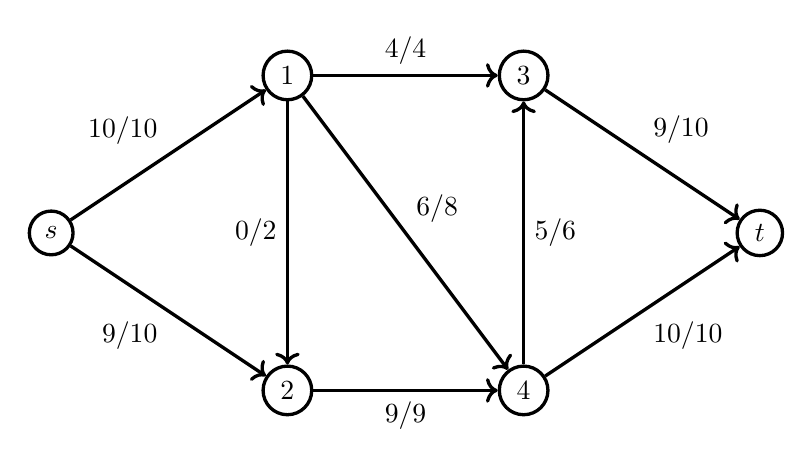
\begin{tikzpicture}
				\node[circle, draw, very thick] (S) at (0,0) {$s$};
				\node[circle, draw, very thick] (1) at (3,2) {$1$};
				\node[circle, draw, very thick] (2) at (3,-2) {$2$};
				\node[circle, draw, very thick] (3) at (6,2) {$3$};
				\node[circle, draw, very thick] (4) at (6,-2) {$4$};
				\node[circle, draw, very thick] (T) at (9,0) {$t$};

				
				\draw[very thick, ->]  (S) -- (1) node[midway,above left] () {$10/10$};
				\draw[very thick, ->]  (S) -- (2) node[midway,below left] () {$9/10$};
				\draw[very thick, ->]  (1) -- (2) node[midway,left] () {$0/2$};
				\draw[very thick, ->]  (1) -- (3) node[midway,above] () {$4/4$};
				\draw[very thick, ->]  (1) -- (4) node[midway,above right] () {$6/8$};
				\draw[very thick, ->]  (2) -- (4) node[midway,below] () {$9/9$};
				\draw[very thick, ->]  (3) -- (T) node[midway,above right] () {$9/10$};
				\draw[very thick, ->]  (4) -- (3) node[midway,right] () {$5/6$};
				\draw[very thick, ->]  (4) -- (T) node[midway,below right] () {$10/10$};
			\end{tikzpicture}
		\end{center}
	\end{frame}
	
	\begin{frame}[plain]{Example}
		\begin{center}
			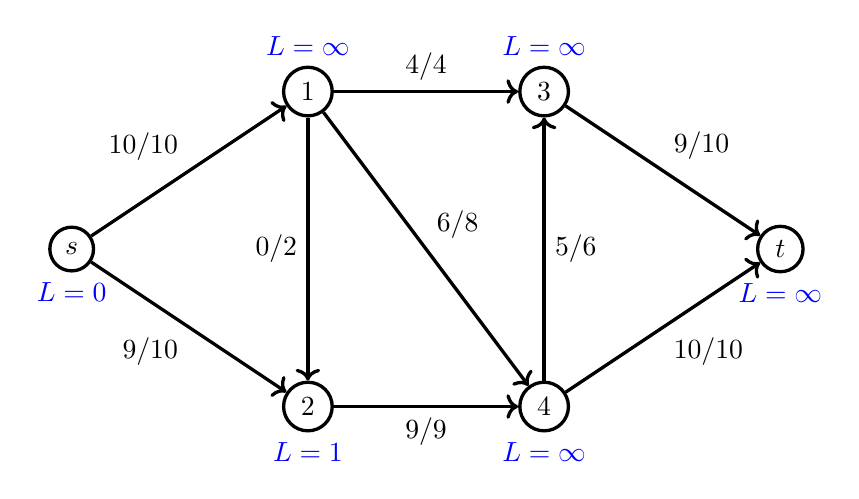
\begin{tikzpicture}
				\node[circle, draw, very thick] (S) at (0,0) {$s$};
				\node[circle, draw, very thick] (1) at (3,2) {$1$};
				\node[circle, draw, very thick] (2) at (3,-2) {$2$};
				\node[circle, draw, very thick] (3) at (6,2) {$3$};
				\node[circle, draw, very thick] (4) at (6,-2) {$4$};
				\node[circle, draw, very thick] (T) at (9,0) {$t$};
				
				\node [below=0cm of S, blue] {$L = 0$};
				\node [below=0cm of 2, blue] {$L = 1$};
				\node [below=0cm of 4, blue] {$L = \infty$};
				\node [above=0cm of 1, blue] {$L = \infty$};
				\node [above=0cm of 3, blue] {$L = \infty$};
				\node [below=0cm of T, blue] {$L = \infty$};
				
				\draw[very thick, ->]  (S) -- (1) node[midway,above left] () {$10/10$};
				\draw[very thick, ->]  (S) -- (2) node[midway,below left] () {$9/10$};
				\draw[very thick, ->]  (1) -- (2) node[midway,left] () {$0/2$};
				\draw[very thick, ->]  (1) -- (3) node[midway,above] () {$4/4$};
				\draw[very thick, ->]  (1) -- (4) node[midway,above right] () {$6/8$};
				\draw[very thick, ->]  (2) -- (4) node[midway,below] () {$9/9$};
				\draw[very thick, ->]  (3) -- (T) node[midway,above right] () {$9/10$};
				\draw[very thick, ->]  (4) -- (3) node[midway,right] () {$5/6$};
				\draw[very thick, ->]  (4) -- (T) node[midway,below right] () {$10/10$};
			\end{tikzpicture}
		\end{center}
	\end{frame}
					
	
	
	\begin{frame}[plain]{Dinic's algorithm}
		\begin{itemize}
			\item Why do this?
			\item Well, now in the layered network every edge out of a vertex $v$ is "toward the sink", so pushing along any one of them is good.
			\item So when pushing flow out of $v$ we just push to the first non-saturated edge. 
			\item Each vertex is given a counter which points to the first non-saturated edge, so we just push to that edge until it's full, then increment if it's full. 
		\end{itemize}
	\end{frame}
	
	\begin{frame}[plain]{Dinic's algorithm}
		\begin{itemize}
			\item How long does making a blocking flow take then?
			\item Each DFS is $\mathcal{O}(n + V))$ where $n$ is the number of increments. 
			\item Each DFS saturates one edge, so we do at most $E$ of them. And we can only increment each vertex $E$ times so the sum of all the $n$ is at most $VE$.
			\item Thus the total time is $\mathcal{O}(VE)$.
			\item Then one can prove this has to be done at most $V$ times as $L(t)$ increases each time (slightly technical, we omit it here)
		\end{itemize}
	\end{frame}
	
	\begin{frame}[plain]{Dinic's algorithm}
		\begin{itemize}
			\item Thus the total time complexity is $\mathcal{O}(V^2E)$, an improvement over $\mathcal{O}(VE^2)$.
			\item But I promised $\mathcal{O}(E\sqrt{V})$?
			\item Well, if all capacities are $1$ then each layered network will take $\mathcal{O}(E)$ since each edge is only considered once.
			\item One can also prove that if all capacities are $1$ there are at most $\sqrt{E}$ phases.
			\item If each vertex has either only 1 in-edge or only 1-out edge, then this can be improved to at most $\sqrt{V}$ phases.
		\end{itemize}
	\end{frame}
	
	\begin{frame}[plain, fragile]{Implementation - part 1}
		\begin{scriptsize}
		\begin{minted}{cpp}
struct FlowEdge {
	int v, u;
	long long cap, flow = 0;
	FlowEdge(int v, int u, long long cap) : v(v), u(u), cap(cap) {}
};

struct Dinic {
	const long long flow_inf = 1e18;
	vector<FlowEdge> edges;
	vector<vector<int>> adj;
	int n, m = 0;
	int s, t;
	vector<int> level, ptr;
	queue<int> q;
	
	Dinic(int n, int s, int t) : n(n), s(s), t(t) {
		adj.resize(n);
		level.resize(n);
		ptr.resize(n);
	}
		\end{minted}
		\end{scriptsize}
	\end{frame}
	
	\begin{frame}[plain, fragile]{Implementation - part 2}
		\begin{scriptsize}
			\begin{minted}{cpp}
void add_edge(int v, int u, long long cap) {
	edges.emplace_back(v, u, cap);
	edges.emplace_back(u, v, 0);
	adj[v].push_back(m);
	adj[u].push_back(m + 1);
	m += 2;
}
bool bfs() {
	while (!q.empty()) {
		int v = q.front();
		q.pop();
		for (int id : adj[v]) {
			if (edges[id].cap == edges[id].flow)
			    continue;
			if (level[edges[id].u] != -1)
			    continue;
			level[edges[id].u] = level[v] + 1;
			q.push(edges[id].u);
		}
	}
	return level[t] != -1;
}
				\end{minted}
			\end{scriptsize}
		\end{frame}
		
	\begin{frame}[plain, fragile]{Implementation - part 3}
		\begin{scriptsize}
			\begin{minted}{cpp}
long long dfs(int v, long long pushed) {
	if (pushed == 0)
	    return 0;
	if (v == t)
	    return pushed;
	for (int& cid = ptr[v]; cid < (int)adj[v].size(); cid++) {
		int id = adj[v][cid];
		int u = edges[id].u;
		if (level[v] + 1 != level[u])
		    continue;
		long long tr = dfs(u, 
                    min(pushed, edges[id].cap - edges[id].flow));
		if (tr == 0)
		    continue;
		edges[id].flow += tr;
		edges[id ^ 1].flow -= tr;
		return tr;
	}
	return 0;
}
			\end{minted}
		\end{scriptsize}
	\end{frame}
	
	\begin{frame}[plain, fragile]{Implementation - part 4}
		\begin{scriptsize}
			\begin{minted}{cpp}
	long long flow() {
		long long f = 0;
		while (true) {
			fill(level.begin(), level.end(), -1);
			level[s] = 0;
			q.push(s);
			if (!bfs())
			    break;
			fill(ptr.begin(), ptr.end(), 0);
			while (long long pushed = dfs(s, flow_inf)) {
				f += pushed;
			}
		}
		return f;
	}
};
			\end{minted}
		\end{scriptsize}
	\end{frame}
	
	\begin{frame}[plain]{MCMF}
		\begin{itemize}
			\item Last algorithm of the day.
			\item What if not all flow is created equal?
			\item It costs much more to send something from $A$ to $B$ than from $A$ to $C$ perhaps
			\item How could we modify Ford-Fulkerson to do this?
		\end{itemize}
	\end{frame}
	
	\begin{frame}[plain]{MCMF}
		\begin{itemize}
			\item Well we could simply take the shortest (cost) path each time instead of the shortest (edges) path each time.
			\item This simply works! (Try to reason why)
			\item If all the costs are $\geq 0$ we can use Dijkstra, otherwise Bellman-Ford is needed (or Johnson's, since negative cycles make the problem undefined anyway)
			\item Only thing to be careful about is to make the reverse edge have cost $-c$ if the original edge has cost $c$, since we want things to cancel
		\end{itemize}
	\end{frame}
	
	
	\begin{frame}[plain]{Hungarian}
		\begin{itemize}
			\item In the case of bipartite matchings where we want maximum/minimum weight, then MCMF will solve it, but there is a better solution
			\item We won't cover it in detail here, but it's known as the Hungarian algorithm or Kuhn-Munkres algorithm
		\end{itemize}
	\end{frame}
\end{document}


